\documentclass[11pt, letterpaper]{article}

% Fonts and Encoding
\usepackage[utf8]{inputenc}
\usepackage[T1]{fontenc}
\usepackage{lmodern} % High-quality Latin Modern vector font

% Math and Symbols
\usepackage{amsmath, amssymb, amsthm, amsfonts, mathrsfs, mathtools}

% Layout and Geometry
\usepackage{geometry}
\geometry{letterpaper, margin=1in}
\setlength{\parindent}{0pt}
\setlength{\parskip}{0.6em}

% Formatting and Graphics
\usepackage{graphicx, xcolor, enumitem, booktabs, array, tabularx}

% TikZ for Illustrations
\usepackage{tikz}
\usetikzlibrary{arrows.meta, positioning, shapes.geometric, calc, backgrounds, matrix}

% Clickable Links and TOC
\usepackage{hyperref}
\hypersetup{
    colorlinks=true,
    linkcolor=blue,
    filecolor=magenta,      
    urlcolor=cyan,
    pdftitle={Mastering Linear Algebra: Diagonalization Problem Sets and Solutions},
}

% Theorem Environments
\newtheorem{theorem}{Theorem}[section]
\newtheorem{lemma}[theorem]{Lemma}
\newtheorem{proposition}[theorem]{Proposition}
\newtheorem{corollary}[theorem]{Corollary}
\theoremstyle{definition}
\newtheorem{definition}{Definition}[section]
\newtheorem{axiom}{Axiom}[section]
\newtheorem{example}{Example}[section]
\theoremstyle{remark}
\newtheorem{remark}{Remark}[section]

% Custom Commands (Enforced standard notation)
\newcommand{\R}{\mathbb{R}}
\newcommand{\N}{\mathbb{N}}
\newcommand{\Z}{\mathbb{Z}}
\newcommand{\Q}{\mathbb{Q}}
\newcommand{\E}{\mathbb{E}}
\newcommand{\Prob}{\mathbb{P}}
\newcommand{\F}{\mathcal{F}}

\title{Mastering Linear Algebra: Diagonalization Problem Sets and Solutions}
\author{Tashfeen Omran}
\date{November 16, 2026}

\begin{document}

\maketitle
\tableofcontents
\newpage

\section{Concept Checklist and Question Mapping}

This section provides a complete concept checklist and question mapping for \textbf{Diagonalization}, aligned with every core formula, algebraic technique, theorem, conceptual pitfall, diagnostic flaw, and real-world application (linear differential equations, quantitative finance, and machine learning). The 30 problems are weighted deliberately so that foundational mechanics receive solid reinforcement while greater emphasis is placed on higher-difficulty topics—namely full $3 \times 3$ diagonalization, parametric and defective matrix analysis, and decoupling in applied dynamical models.

\subsection{Essential Formulas Reference}

\renewcommand{\arraystretch}{1.5}
\begin{tabularx}{\textwidth}{l >{$\displaystyle}l<{$} X}
\toprule
\textbf{Concept} & \multicolumn{1}{l}{\textbf{Canonical Formula}} & \textbf{Key Requirement and Context} \\
\midrule
Diagonalization & A = P D P^{-1} & $P$ is invertible (eigenvectors as columns) and $D$ is strictly diagonal (eigenvalues in matching order). \\
Matrix Powers & A^{k} = P D^{k} P^{-1} & Follows from telescoping cancellation; $D^{k}$ raises each diagonal entry to power $k$. \\
Characteristic Equation & \det(A - \lambda I) = 0 & Yields eigenvalues $\lambda$ and their algebraic multiplicities; avoid $ad + bc$ sign errors in $2 \times 2$ determinants. \\
Eigenspace Basis & \operatorname{Nul}(A - \lambda I) & Found via Gaussian elimination; geometric multiplicity must equal algebraic multiplicity for all $\lambda$ (Theorem 7). \\
\bottomrule
\end{tabularx}

\subsection{Complete Concept Checklist and Question Mapping}

\renewcommand{\arraystretch}{1.5}
\begin{tabularx}{\textwidth}{l X X c p{3.1cm}}
\toprule
\textbf{ID} & \textbf{Concept / Problem Type} & \textbf{Key Techniques, Theorems, and Pitfalls} & \textbf{Weight} & \textbf{Relevant Questions} \\
\midrule
C1 & Matrix Powers via Factorization ($A^{k} = PD^{k}P^{-1}$) & $2 \times 2$ inverse with $1/\det(P)$, telescoping cancellation, symbolic powers, asymptotic limits. & 4 (13.3\%) & \textbf{Primary:} \hyperref[prob:1]{1}, \hyperref[prob:2]{2}, \hyperref[prob:3]{3}, \hyperref[prob:4]{4}\newline \textbf{Related:} \hyperref[prob:20]{20}, \hyperref[prob:23]{23}, \hyperref[prob:29]{29} \\
\addlinespace[3pt]
C2 & Triangular Shortcuts and Fraction Avoidance & Reading $\lambda$ directly off triangular diagonals; scaling free variables to avoid fractions in RREF. & 2 (6.7\%) & \textbf{Primary:} \hyperref[prob:5]{5}, \hyperref[prob:6]{6}\newline \textbf{Related:} \hyperref[prob:8]{8}, \hyperref[prob:11]{11}, \hyperref[prob:14]{14}, \hyperref[prob:15]{15} \\
\addlinespace[3pt]
C3 & Full Diagonalization ($2 \times 2$ and $3 \times 3$) & Solving $\det(A-\lambda I)=0$, computing bases for $\operatorname{Nul}(A-\lambda I)$, handling $\lambda = 0$ and repeated $\lambda$. & 5 (16.7\%) & \textbf{Primary:} \hyperref[prob:7]{7}, \hyperref[prob:8]{8}, \hyperref[prob:9]{9}, \hyperref[prob:10]{10}, \hyperref[prob:11]{11}\newline \textbf{Related:} \hyperref[prob:4]{4}, \hyperref[prob:22]{22}--\hyperref[prob:26]{26} \\
\addlinespace[3pt]
C4 & Conceptual Theorems and Parametric Analysis & Theorems 5, 6, 7; similarity vs.\ diagonalizability; rank-nullity; parameter conditions for diagonalizability. & 4 (13.3\%) & \textbf{Primary:} \hyperref[prob:12]{12}, \hyperref[prob:13]{13}, \hyperref[prob:14]{14}, \hyperref[prob:15]{15}\newline \textbf{Related:} \hyperref[prob:21]{21}, \hyperref[prob:30]{30} \\
\addlinespace[3pt]
C5 & Defective Matrices and Jordan Canonical Form & Algebraic vs.\ geometric multiplicity gap, $\det(P)=0$ failure, nilpotent blocks $A = \lambda I + N$ and $J$. & 3 (10.0\%) & \textbf{Primary:} \hyperref[prob:16]{16}, \hyperref[prob:17]{17}, \hyperref[prob:18]{18}\newline \textbf{Related:} \hyperref[prob:14]{14}, \hyperref[prob:15]{15}, \hyperref[prob:30]{30} \\
\addlinespace[3pt]
C6 & Change of Basis, Matrix Roots, and Structural Identities & Computing $A^{k}\mathbf{x}$ via $[\mathbf{x}]_{\mathcal{B}}$, reconstructing $A$, $A^{-1}$, $\sqrt{A}$, $A^{T}$, and $A+cI$. & 3 (10.0\%) & \textbf{Primary:} \hyperref[prob:19]{19}, \hyperref[prob:20]{20}, \hyperref[prob:21]{21}\newline \textbf{Related:} \hyperref[prob:24]{24}, \hyperref[prob:26]{26} \\
\addlinespace[3pt]
C7 & Applied Decoupling (ODEs, Recurrences, OU, PCA) & Coupled $\mathbf{x}' = A\mathbf{x}$, discrete $\mathbf{x}_{k+1}=A\mathbf{x}_k$, Ornstein-Uhlenbeck SDEs ($\mathbf{Y}_t = P^{-1}\mathbf{X}_t$), PCA variance. & 5 (16.7\%) & \textbf{Primary:} \hyperref[prob:22]{22}, \hyperref[prob:23]{23}, \hyperref[prob:24]{24}, \hyperref[prob:25]{25}, \hyperref[prob:26]{26}\newline \textbf{Related:} \hyperref[prob:4]{4} \\
\addlinespace[3pt]
C8 & Diagnostic Error Analysis (``Find the Flaw'') & Detecting swapped columns in $P$/$D$, $ad+bc$ sign errors, $P^{-1}D^{k}P$ order errors, missing $1/\det(P)$, repeated vectors. & 4 (13.3\%) & \textbf{Primary:} \hyperref[prob:27]{27}, \hyperref[prob:28]{28}, \hyperref[prob:29]{29}, \hyperref[prob:30]{30}\newline \textbf{Related:} \hyperref[prob:12]{12} \\
\bottomrule
\end{tabularx}

\newpage
\section{Problem Sets}

\subsection{Part A: Matrix Powers and Algebraic Factorizations}

\textbf{Problem 1.}\phantomsection\label{prob:1}
Compute $A^{4}$, where $A = PDP^{-1}$ and
\[
P = \begin{bmatrix} 4 & 5 \\ 3 & 4 \end{bmatrix}, \qquad D = \begin{bmatrix} 2 & 0 \\ 0 & -1 \end{bmatrix}.
\]

\textbf{Problem 2.}\phantomsection\label{prob:2}
Let $A = PDP^{-1}$, where
\[
P = \begin{bmatrix} 2 & 1 \\ 1 & 2 \end{bmatrix}, \qquad D = \begin{bmatrix} 1 & 0 \\ 0 & -2 \end{bmatrix}.
\]
Compute $P^{-1}$, and then use the diagonalization to compute $A^{3}$ and $A^{5}$.

\textbf{Problem 3.}\phantomsection\label{prob:3}
Use the factorization $A = PDP^{-1}$ to compute $A^{k}$ for an arbitrary positive integer $k \in \mathbb{Z}^{+}$, where $a, b \in \mathbb{R}$ and
\[
A = \begin{bmatrix} 2b - a & 2(a - b) \\ b - a & 2a - b \end{bmatrix} = \begin{bmatrix} 1 & -2 \\ 1 & -1 \end{bmatrix} \begin{bmatrix} a & 0 \\ 0 & b \end{bmatrix} \begin{bmatrix} -1 & 2 \\ -1 & 1 \end{bmatrix}.
\]

\textbf{Problem 4.}\phantomsection\label{prob:4}
Consider the transition matrix
\[
A = \begin{bmatrix} 3/4 & 1/2 \\ 1/4 & 1/2 \end{bmatrix}.
\]
\begin{enumerate}[label=(\alph*)]
    \item Diagonalize $A$ in the form $A = PDP^{-1}$.
    \item Find a closed-form expression for $A^{k}$ valid for any integer $k \ge 1$.
    \item Compute the steady-state limit $\lim_{k \to \infty} A^{k}$.
\end{enumerate}

\subsection{Part B: Triangular Shortcuts and Full Diagonalization}

\textbf{Problem 5.}\phantomsection\label{prob:5}
Diagonalize the lower triangular matrix
\[
A = \begin{bmatrix} 3 & 0 \\ 8 & -1 \end{bmatrix},
\]
if possible, by explicitly constructing $P$ and $D$ such that $A = PDP^{-1}$.

\textbf{Problem 6.}\phantomsection\label{prob:6}
Diagonalize the upper triangular matrix
\[
A = \begin{bmatrix} 2 & 1 & -3 \\ 0 & -1 & 4 \\ 0 & 0 & 5 \end{bmatrix},
\]
choosing integer-valued eigenvectors in $P$ to avoid fractions.

\textbf{Problem 7.}\phantomsection\label{prob:7}
Find the characteristic polynomial, eigenvalues, and corresponding eigenspaces of
\[
A = \begin{bmatrix} 4 & -2 \\ 1 & 1 \end{bmatrix},
\]
and construct matrices $P$ and $D$ such that $A = PDP^{-1}$.

\textbf{Problem 8.}\phantomsection\label{prob:8}
Diagonalize the matrix
\[
A = \begin{bmatrix} -5 & 6 & -2 \\ -8 & 8 & -1 \\ -8 & 6 & 1 \end{bmatrix},
\]
given that its eigenvalues are $\lambda = -1, 2, 3$. Choose integer eigenvectors for the columns of $P$.

\textbf{Problem 9.}\phantomsection\label{prob:9}
Determine all eigenvalues of
\[
A = \begin{bmatrix} 4 & 3 & -3 \\ 3 & 4 & -3 \\ 3 & 3 & -2 \end{bmatrix}
\]
from its characteristic polynomial, and diagonalize $A$ if possible (constructing $P$ and $D$ explicitly).

\textbf{Problem 10.}\phantomsection\label{prob:10}
Diagonalize the matrix
\[
A = \begin{bmatrix} 0 & 1 & -1 \\ -1 & 2 & 1 \\ -2 & 2 & 1 \end{bmatrix}
\]
from scratch without being given its eigenvalues.

\textbf{Problem 11.}\phantomsection\label{prob:11}
Consider the symmetric matrix
\[
A = \begin{bmatrix} 2 & 0 & 1 \\ 0 & 2 & 1 \\ 1 & 1 & 1 \end{bmatrix}.
\]
\begin{enumerate}[label=(\alph*)]
    \item Find all eigenvalues and a basis of integer eigenvectors for each eigenspace, and construct $P$ and $D$ such that $A = PDP^{-1}$.
    \item Is $A$ invertible? Explain clearly why invertibility of $A$ and diagonalizability of $A$ are independent properties.
\end{enumerate}

\subsection{Part C: Conceptual Theorems, Dimensionality, and Parametric Analysis}

\textbf{Problem 12.}\phantomsection\label{prob:12}
Determine whether each of the following statements is \textbf{True} or \textbf{False}, and provide a rigorous mathematical justification (citing a theorem or giving an explicit counterexample):
\begin{enumerate}[label=(\alph*)]
    \item If $A = PBP^{-1}$ for some invertible matrix $P$ and some square matrix $B$, then $A$ is diagonalizable.
    \item Every invertible $n \times n$ matrix is diagonalizable over $\mathbb{R}$.
    \item If an $n \times n$ matrix $A$ has $n$ distinct real eigenvalues, then $A$ is diagonalizable over $\mathbb{R}$.
    \item If an $n \times n$ matrix $A$ is diagonalizable, then $A$ must have $n$ distinct eigenvalues.
\end{enumerate}

\textbf{Problem 13.}\phantomsection\label{prob:13}
Let $A$ be a $6 \times 6$ matrix with exactly three distinct eigenvalues $\lambda_1, \lambda_2, \lambda_3$. Suppose that $\operatorname{rank}(A - \lambda_1 I) = 4$, $\dim\operatorname{Nul}(A - \lambda_2 I) = 3$, and $\lambda_3$ has algebraic multiplicity $1$.
\begin{enumerate}[label=(\alph*)]
    \item Is $A$ diagonalizable? Justify your conclusion using the Rank-Nullity Theorem and the Diagonalization Theorem (Theorem 7).
    \item Deduce the exact algebraic multiplicities of $\lambda_1$ and $\lambda_2$.
\end{enumerate}

\textbf{Problem 14.}\phantomsection\label{prob:14}
Find all real values of the parameter $c \in \mathbb{R}$ for which the matrix
\[
A = \begin{bmatrix} 2 & c & 1 \\ 0 & 2 & 3 \\ 0 & 0 & 5 \end{bmatrix}
\]
is diagonalizable over $\mathbb{R}$. For every such value of $c$, find an invertible matrix $P$ and a diagonal matrix $D$ satisfying $A = PDP^{-1}$.

\textbf{Problem 15.}\phantomsection\label{prob:15}
Find all real values of the parameter $k \in \mathbb{R}$ for which the matrix
\[
A = \begin{bmatrix} 2 & 1 & 1 \\ 0 & k & 2 \\ 0 & 0 & 2 \end{bmatrix}
\]
is diagonalizable over $\mathbb{R}$. For each such value of $k$, construct $P$ and $D$ such that $A = PDP^{-1}$.

\subsection{Part D: Defective Matrices and Jordan Canonical Form}

\textbf{Problem 16.}\phantomsection\label{prob:16}
Show that the matrix
\[
A = \begin{bmatrix} 5 & -1 \\ 1 & 3 \end{bmatrix}
\]
is defective and therefore cannot be diagonalized. State the algebraic multiplicity and geometric multiplicity of its eigenvalue, and write down the Jordan Canonical Form $J$ of $A$.

\textbf{Problem 17.}\phantomsection\label{prob:17}
Determine whether the $3 \times 3$ matrix
\[
A = \begin{bmatrix} 2 & 1 & 0 \\ 0 & 2 & 0 \\ 1 & -1 & 3 \end{bmatrix}
\]
is diagonalizable. If not, identify the eigenvalue responsible for the failure and compute its algebraic and geometric multiplicities.

\textbf{Problem 18.}\phantomsection\label{prob:18}
Consider the $3 \times 3$ Jordan block
\[
A = \begin{bmatrix} 3 & 1 & 0 \\ 0 & 3 & 1 \\ 0 & 0 & 3 \end{bmatrix}.
\]
\begin{enumerate}[label=(\alph*)]
    \item Find the algebraic and geometric multiplicities of $\lambda = 3$, and explain why $A$ is defective.
    \item Write $A = 3I + N$, verify that $N^{3} = 0$, and use the Binomial Theorem (valid because $3I$ and $N$ commute) to find a closed-form expression for $A^{k}$ for all integers $k \ge 1$. Contrast this behavior with the powers of a diagonalizable matrix.
\end{enumerate}

\subsection{Part E: Change of Basis, Matrix Roots, and Structural Properties}

\textbf{Problem 19.}\phantomsection\label{prob:19}
Suppose a $2 \times 2$ matrix $A$ has eigenvectors $\mathbf{v}_1 = \begin{bmatrix} 2 \\ 1 \end{bmatrix}$ corresponding to $\lambda_1 = 4$ and $\mathbf{v}_2 = \begin{bmatrix} 1 \\ -1 \end{bmatrix}$ corresponding to $\lambda_2 = 1$.
\begin{enumerate}[label=(\alph*)]
    \item Without first reconstructing the matrix $A$, compute $A\mathbf{x}$ and $A^{3}\mathbf{x}$ for $\mathbf{x} = \begin{bmatrix} 5 \\ 1 \end{bmatrix}$ by finding the eigenbasis coordinate vector $[\mathbf{x}]_{\mathcal{B}} = P^{-1}\mathbf{x}$.
    \item Explicitly reconstruct $A = PDP^{-1}$ and verify your answers to part (a).
\end{enumerate}

\textbf{Problem 20.}\phantomsection\label{prob:20}
Suppose a $2 \times 2$ matrix $A$ has diagonalization $A = PDP^{-1}$ with
\[
P = \begin{bmatrix} 1 & 2 \\ 1 & 3 \end{bmatrix}, \qquad D = \begin{bmatrix} 4 & 0 \\ 0 & 9 \end{bmatrix}.
\]
\begin{enumerate}[label=(\alph*)]
    \item Compute $A$ and use the factorization $A^{-1} = PD^{-1}P^{-1}$ to compute $A^{-1}$.
    \item Find a matrix square root $B$ (having positive eigenvalues) such that $B^{2} = A$ via $B = PD^{1/2}P^{-1}$, and verify by direct multiplication that $B^{2} = A$.
\end{enumerate}

\textbf{Problem 21.}\phantomsection\label{prob:21}
Suppose $A$ is a diagonalizable $n \times n$ matrix with factorization $A = PDP^{-1}$.
\begin{enumerate}[label=(\alph*)]
    \item Prove that the transpose $A^{T}$ is also diagonalizable, and express its diagonalization explicitly in terms of $P$ and $D$.
    \item Prove that for any scalar $c \in \mathbb{R}$, the shifted matrix $A + cI$ is diagonalizable using the \emph{same} eigenvector matrix $P$.
    \item Provide an explicit $2 \times 2$ counterexample showing that $A^{2}$ can be diagonalizable even when $A$ itself is \emph{not} diagonalizable.
\end{enumerate}

\subsection{Part F: Applied Modeling in Differential Equations, Quantitative Finance, and Machine Learning}

\textbf{Problem 22.}\phantomsection\label{prob:22}
Solve the coupled system of linear ordinary differential equations
\[
\begin{cases}
x_{1}'(t) = 2x_{1}(t) + 3x_{2}(t), \\
x_{2}'(t) = 2x_{1}(t) + x_{2}(t),
\end{cases}
\qquad \mathbf{x}(0) = \begin{bmatrix} 1 \\ 4 \end{bmatrix},
\]
by diagonalizing the coefficient matrix $A$ and applying the change of basis $\mathbf{y}(t) = P^{-1}\mathbf{x}(t)$ to decouple the system into independent scalar equations.

\textbf{Problem 23.}\phantomsection\label{prob:23}
Consider the second-order linear recurrence relation $u_{k+2} = 5u_{k+1} - 6u_{k}$ with initial values $u_{0} = 2$ and $u_{1} = 5$.
\begin{enumerate}[label=(\alph*)]
    \item Rewrite this recurrence as a first-order matrix dynamical system $\mathbf{x}_{k+1} = A\mathbf{x}_{k}$, where $\mathbf{x}_{k} = \begin{bmatrix} u_{k+1} \\ u_{k} \end{bmatrix}$.
    \item Diagonalize $A$ and use $\mathbf{x}_{k} = A^{k}\mathbf{x}_{0} = PD^{k}P^{-1}\mathbf{x}_{0}$ to derive a closed-form formula for $u_{k}$ for all integers $k \ge 0$.
\end{enumerate}

\textbf{Problem 24.}\phantomsection\label{prob:24}
In statistical arbitrage, the log-prices $\mathbf{X}_{t} = \begin{bmatrix} X_{t}^{(1)} \\ X_{t}^{(2)} \end{bmatrix}$ of two cointegrated assets follow a multidimensional Ornstein-Uhlenbeck stochastic differential equation:
\[
d\mathbf{X}_{t} = \Theta(\boldsymbol{\mu} - \mathbf{X}_{t})\,dt + \Sigma\,d\mathbf{W}_{t},
\]
where $\mathbf{W}_{t}$ is a $2$-dimensional standard Wiener process and
\[
\Theta = \begin{bmatrix} 5 & -2 \\ -2 & 2 \end{bmatrix}, \qquad \boldsymbol{\mu} = \begin{bmatrix} 4 \\ 3 \end{bmatrix}, \qquad \Sigma = \begin{bmatrix} 1 & 0 \\ 0 & 1 \end{bmatrix}.
\]
\begin{enumerate}[label=(\alph*)]
    \item Diagonalize the mean-reversion matrix as $\Theta = P\Lambda P^{-1}$, ordering the eigenvalues so that $\lambda_{1} < \lambda_{2}$.
    \item Define the synthetic portfolio vector $\mathbf{Y}_{t} = P^{-1}\mathbf{X}_{t}$. Apply It\^{o}'s Lemma ($d\mathbf{Y}_{t} = P^{-1}\,d\mathbf{X}_{t}$) to write the decoupled scalar SDEs for $dY_{t}^{(1)}$ and $dY_{t}^{(2)}$ explicitly.
    \item Which synthetic portfolio mean-reverts faster, and what is its mean-reversion half-life $\tau_{1/2} = \frac{\ln 2}{\lambda}$?
\end{enumerate}

\textbf{Problem 25.}\phantomsection\label{prob:25}
Consider a two-asset Ornstein-Uhlenbeck model $d\mathbf{X}_{t} = \Theta(\boldsymbol{\mu} - \mathbf{X}_{t})\,dt + \Sigma\,d\mathbf{W}_{t}$ with non-symmetric drift matrix and correlated volatility:
\[
\Theta = \begin{bmatrix} 4 & -1 \\ 2 & 1 \end{bmatrix}, \qquad \boldsymbol{\mu} = \begin{bmatrix} 3 \\ 4 \end{bmatrix}, \qquad \Sigma = \begin{bmatrix} 2 & 1 \\ 1 & 2 \end{bmatrix}.
\]
\begin{enumerate}[label=(\alph*)]
    \item Diagonalize $\Theta = P\Lambda P^{-1}$ and explain why the eigenvalues confirm that the system is mean-reverting (stable).
    \item Transform the SDE to the eigenbasis $\mathbf{Y}_{t} = P^{-1}\mathbf{X}_{t}$ and compute the decoupled drift term $\Lambda(P^{-1}\boldsymbol{\mu} - \mathbf{Y}_{t})$ and transformed diffusion matrix $P^{-1}\Sigma$.
\end{enumerate}

\textbf{Problem 26.}\phantomsection\label{prob:26}
In Principal Component Analysis (PCA), a centered dataset in $\mathbb{R}^{2}$ has sample covariance matrix
\[
C = \begin{bmatrix} 5 & 2 \\ 2 & 2 \end{bmatrix}.
\]
\begin{enumerate}[label=(\alph*)]
    \item Diagonalize $C = PDP^{-1}$ such that the columns of $P$ are \emph{unit} eigenvectors $\{\mathbf{u}_{1}, \mathbf{u}_{2}\}$ ordered with $\lambda_{1} \ge \lambda_{2}$.
    \item What percentage of the total variance $\operatorname{tr}(C) = \lambda_{1} + \lambda_{2}$ is captured by the first principal component $\mathbf{u}_{1}$?
    \item Compute the principal component coordinates $[\mathbf{x}]_{\mathcal{B}} = P^{-1}\mathbf{x}$ of the observation $\mathbf{x} = \begin{bmatrix} 3 \\ 1 \end{bmatrix}$, and explain why $P^{-1} = P^{T}$ holds here.
\end{enumerate}

\subsection{Part G: Diagnostic Error Analysis (``Find the Flaw'')}

\textbf{Problem 27.}\phantomsection\label{prob:27}
Act as the grader for the following attempt to compute $A^{2}$ for $A = \begin{bmatrix} 1 & 2 \\ 4 & 3 \end{bmatrix}$ via diagonalization:
\begin{quote}
\emph{Student's Solution:} Solving $\det(A - \lambda I) = 0$ gives $\lambda_{1} = 5$ with eigenvector $\mathbf{v}_{1} = \begin{bmatrix} 1 \\ 2 \end{bmatrix}$ and $\lambda_{2} = -1$ with eigenvector $\mathbf{v}_{2} = \begin{bmatrix} 1 \\ -1 \end{bmatrix}$. Forming
\[
P = \begin{bmatrix} 1 & 1 \\ -1 & 2 \end{bmatrix}, \qquad D = \begin{bmatrix} 5 & 0 \\ 0 & -1 \end{bmatrix},
\]
and inverting $P$ gives $P^{-1} = \begin{bmatrix} 2 & -1 \\ 1 & 1 \end{bmatrix}$. Hence
\[
A^{2} = PD^{2}P^{-1} = \begin{bmatrix} 1 & 1 \\ -1 & 2 \end{bmatrix} \begin{bmatrix} 25 & 0 \\ 0 & 1 \end{bmatrix} \begin{bmatrix} 2 & -1 \\ 1 & 1 \end{bmatrix} = \begin{bmatrix} 51 & -24 \\ -48 & 27 \end{bmatrix}.
\]
\end{quote}
Identify \textbf{two} distinct flaws in the student's work, explain why each is incorrect, and compute the correct diagonalization and value of $A^{2}$.

\textbf{Problem 28.}\phantomsection\label{prob:28}
Act as the grader for the following attempt to diagonalize $A = \begin{bmatrix} 3 & 2 \\ 5 & 0 \end{bmatrix}$ over $\mathbb{R}$:
\begin{quote}
\emph{Student's Solution:} The characteristic equation is $\det(A - \lambda I) = (3 - \lambda)(-\lambda) + (2)(5) = \lambda^{2} - 3\lambda + 10 = 0$. Since the discriminant is $(-3)^{2} - 4(1)(10) = -31 < 0$, $A$ has no real eigenvalues and therefore cannot be diagonalized over $\mathbb{R}$.
\end{quote}
Identify the flaw, explain why it is incorrect in one sentence, and find the correct eigenvalues and diagonalization $P, D$.

\textbf{Problem 29.}\phantomsection\label{prob:29}
Act as the grader for the following computation of $A^{3}$ given $A = PDP^{-1}$ with $P = \begin{bmatrix} 1 & 1 \\ 0 & 1 \end{bmatrix}$ and $D = \begin{bmatrix} 2 & 0 \\ 0 & 3 \end{bmatrix}$:
\begin{quote}
\emph{Student's Solution:} Raising the factorization to the third power gives
\[
A^{3} = P^{-1}D^{3}P = \begin{bmatrix} 1 & -1 \\ 0 & 1 \end{bmatrix} \begin{bmatrix} 8 & 0 \\ 0 & 27 \end{bmatrix} \begin{bmatrix} 1 & 1 \\ 0 & 1 \end{bmatrix} = \begin{bmatrix} 8 & -19 \\ 0 & 27 \end{bmatrix}.
\]
\end{quote}
Identify the flaw, explain why it is incorrect in one sentence, and compute the correct matrix $A^{3}$.

\textbf{Problem 30.}\phantomsection\label{prob:30}
Act as the grader for the following attempt to determine whether $A = \begin{bmatrix} 4 & 1 \\ -1 & 2 \end{bmatrix}$ is diagonalizable:
\begin{quote}
\emph{Student's Solution:} We find $\det(A - \lambda I) = (4-\lambda)(2-\lambda) + 1 = (\lambda - 3)^{2} = 0$, so $\lambda = 3$ has algebraic multiplicity $2$. Solving $(A - 3I)\mathbf{x} = \mathbf{0}$ yields $\mathbf{v}_{1} = \begin{bmatrix} 1 \\ -1 \end{bmatrix}$. Choosing a second eigenvector $\mathbf{v}_{2} = \begin{bmatrix} -2 \\ 2 \end{bmatrix}$ gives
\[
P = \begin{bmatrix} 1 & -2 \\ -1 & 2 \end{bmatrix}, \qquad D = \begin{bmatrix} 3 & 0 \\ 0 & 3 \end{bmatrix},
\]
so $A$ is diagonalizable.
\end{quote}
Identify the flaw, explain why it is incorrect, and state the correct conclusion regarding the diagonalizability of $A$.

\newpage
\section{Detailed Solutions}

\subsection{Solutions to Part A: Matrix Powers and Algebraic Factorizations}

\textbf{Problem 1 (Original Statement):}
Compute $A^{4}$, where $A = PDP^{-1}$ and
\[
P = \begin{bmatrix} 4 & 5 \\ 3 & 4 \end{bmatrix}, \qquad D = \begin{bmatrix} 2 & 0 \\ 0 & -1 \end{bmatrix}.
\]

\textbf{Solution:}
First, compute $P^{-1}$ using the $2 \times 2$ inverse formula. Since $\det(P) = (4)(4) - (5)(3) = 16 - 15 = 1$, we obtain:
\[
P^{-1} = \frac{1}{1}\begin{bmatrix} 4 & -5 \\ -3 & 4 \end{bmatrix} = \begin{bmatrix} 4 & -5 \\ -3 & 4 \end{bmatrix}.
\]
Next, compute $D^{4}$ by raising each diagonal entry to the $4$th power:
\[
D^{4} = \begin{bmatrix} 2^{4} & 0 \\ 0 & (-1)^{4} \end{bmatrix} = \begin{bmatrix} 16 & 0 \\ 0 & 1 \end{bmatrix}.
\]
Using the telescoping matrix power formula $A^{4} = PD^{4}P^{-1}$, first compute $PD^{4}$:
\[
PD^{4} = \begin{bmatrix} 4 & 5 \\ 3 & 4 \end{bmatrix} \begin{bmatrix} 16 & 0 \\ 0 & 1 \end{bmatrix} = \begin{bmatrix} 4(16) + 5(0) & 4(0) + 5(1) \\ 3(16) + 4(0) & 3(0) + 4(1) \end{bmatrix} = \begin{bmatrix} 64 & 5 \\ 48 & 4 \end{bmatrix}.
\]
Now multiply on the right by $P^{-1}$:
\[
A^{4} = (PD^{4})P^{-1} = \begin{bmatrix} 64 & 5 \\ 48 & 4 \end{bmatrix} \begin{bmatrix} 4 & -5 \\ -3 & 4 \end{bmatrix} = \begin{bmatrix} 256 - 15 & -320 + 20 \\ 192 - 12 & -240 + 16 \end{bmatrix} = \begin{bmatrix} 241 & -300 \\ 180 & -224 \end{bmatrix}.
\]
\textbf{Final Answer:} $A^{4} = \begin{bmatrix} 241 & -300 \\ 180 & -224 \end{bmatrix}$.

\vspace{0.8em}
\textbf{Problem 2 (Original Statement):}
Let $A = PDP^{-1}$, where
\[
P = \begin{bmatrix} 2 & 1 \\ 1 & 2 \end{bmatrix}, \qquad D = \begin{bmatrix} 1 & 0 \\ 0 & -2 \end{bmatrix}.
\]
Compute $P^{-1}$, and then use the diagonalization to compute $A^{3}$ and $A^{5}$.

\textbf{Solution:}
Compute the determinant of $P$: $\det(P) = (2)(2) - (1)(1) = 3$. Applying the $2 \times 2$ inverse formula (including the factor $1/\det(P)$):
\[
P^{-1} = \frac{1}{3}\begin{bmatrix} 2 & -1 \\ -1 & 2 \end{bmatrix}.
\]
For $A^{3} = PD^{3}P^{-1}$, we first compute $D^{3} = \begin{bmatrix} 1^{3} & 0 \\ 0 & (-2)^{3} \end{bmatrix} = \begin{bmatrix} 1 & 0 \\ 0 & -8 \end{bmatrix}$, and then:
\[
PD^{3} = \begin{bmatrix} 2 & 1 \\ 1 & 2 \end{bmatrix}\begin{bmatrix} 1 & 0 \\ 0 & -8 \end{bmatrix} = \begin{bmatrix} 2 & -8 \\ 1 & -16 \end{bmatrix},
\]
\[
A^{3} = \frac{1}{3}\begin{bmatrix} 2 & -8 \\ 1 & -16 \end{bmatrix}\begin{bmatrix} 2 & -1 \\ -1 & 2 \end{bmatrix} = \frac{1}{3}\begin{bmatrix} 4 + 8 & -2 - 16 \\ 2 + 16 & -1 - 32 \end{bmatrix} = \frac{1}{3}\begin{bmatrix} 12 & -18 \\ 18 & -33 \end{bmatrix} = \begin{bmatrix} 4 & -6 \\ 6 & -11 \end{bmatrix}.
\]
Similarly, for $A^{5} = PD^{5}P^{-1}$, we have $D^{5} = \begin{bmatrix} 1^{5} & 0 \\ 0 & (-2)^{5} \end{bmatrix} = \begin{bmatrix} 1 & 0 \\ 0 & -32 \end{bmatrix}$, so:
\[
PD^{5} = \begin{bmatrix} 2 & 1 \\ 1 & 2 \end{bmatrix}\begin{bmatrix} 1 & 0 \\ 0 & -32 \end{bmatrix} = \begin{bmatrix} 2 & -32 \\ 1 & -64 \end{bmatrix},
\]
\[
A^{5} = \frac{1}{3}\begin{bmatrix} 2 & -32 \\ 1 & -64 \end{bmatrix}\begin{bmatrix} 2 & -1 \\ -1 & 2 \end{bmatrix} = \frac{1}{3}\begin{bmatrix} 4 + 32 & -2 - 64 \\ 2 + 64 & -1 - 128 \end{bmatrix} = \frac{1}{3}\begin{bmatrix} 36 & -66 \\ 66 & -129 \end{bmatrix} = \begin{bmatrix} 12 & -22 \\ 22 & -43 \end{bmatrix}.
\]
\textbf{Final Answer:} $P^{-1} = \frac{1}{3}\begin{bmatrix} 2 & -1 \\ -1 & 2 \end{bmatrix}$, $A^{3} = \begin{bmatrix} 4 & -6 \\ 6 & -11 \end{bmatrix}$, and $A^{5} = \begin{bmatrix} 12 & -22 \\ 22 & -43 \end{bmatrix}$.

\vspace{0.8em}
\textbf{Problem 3 (Original Statement):}
Use the factorization $A = PDP^{-1}$ to compute $A^{k}$ for an arbitrary positive integer $k \in \mathbb{Z}^{+}$, where $a, b \in \mathbb{R}$ and
\[
A = \begin{bmatrix} 2b - a & 2(a - b) \\ b - a & 2a - b \end{bmatrix} = \begin{bmatrix} 1 & -2 \\ 1 & -1 \end{bmatrix} \begin{bmatrix} a & 0 \\ 0 & b \end{bmatrix} \begin{bmatrix} -1 & 2 \\ -1 & 1 \end{bmatrix}.
\]

\textbf{Solution:}
Here $P = \begin{bmatrix} 1 & -2 \\ 1 & -1 \end{bmatrix}$, $D = \begin{bmatrix} a & 0 \\ 0 & b \end{bmatrix}$, and $P^{-1} = \begin{bmatrix} -1 & 2 \\ -1 & 1 \end{bmatrix}$. Using $A^{k} = PD^{k}P^{-1}$ with $D^{k} = \begin{bmatrix} a^{k} & 0 \\ 0 & b^{k} \end{bmatrix}$:
\[
PD^{k} = \begin{bmatrix} 1 & -2 \\ 1 & -1 \end{bmatrix}\begin{bmatrix} a^{k} & 0 \\ 0 & b^{k} \end{bmatrix} = \begin{bmatrix} a^{k} & -2b^{k} \\ a^{k} & -b^{k} \end{bmatrix}.
\]
Multiplying on the right by $P^{-1}$ yields:
\[
A^{k} = \begin{bmatrix} a^{k} & -2b^{k} \\ a^{k} & -b^{k} \end{bmatrix}\begin{bmatrix} -1 & 2 \\ -1 & 1 \end{bmatrix} = \begin{bmatrix} -a^{k} + 2b^{k} & 2a^{k} - 2b^{k} \\ -a^{k} + b^{k} & 2a^{k} - b^{k} \end{bmatrix} = \begin{bmatrix} 2b^{k} - a^{k} & 2(a^{k} - b^{k}) \\ b^{k} - a^{k} & 2a^{k} - b^{k} \end{bmatrix}.
\]
Notice that setting $k = 1$ immediately recovers the original matrix $A$.

\textbf{Final Answer:} $A^{k} = \begin{bmatrix} 2b^{k} - a^{k} & 2(a^{k} - b^{k}) \\ b^{k} - a^{k} & 2a^{k} - b^{k} \end{bmatrix}$.

\vspace{0.8em}
\textbf{Problem 4 (Original Statement):}
Consider the transition matrix
\[
A = \begin{bmatrix} 3/4 & 1/2 \\ 1/4 & 1/2 \end{bmatrix}.
\]
\begin{enumerate}[label=(\alph*)]
    \item Diagonalize $A$ in the form $A = PDP^{-1}$.
    \item Find a closed-form expression for $A^{k}$ valid for any integer $k \ge 1$.
    \item Compute the steady-state limit $\lim_{k \to \infty} A^{k}$.
\end{enumerate}

\textbf{Solution:}
\begin{enumerate}[label=(\alph*)]
    \item Compute the characteristic polynomial:
    \[
    \det(A - \lambda I) = \left(\frac{3}{4} - \lambda\right)\left(\frac{1}{2} - \lambda\right) - \left(\frac{1}{2}\right)\left(\frac{1}{4}\right) = \lambda^{2} - \frac{5}{4}\lambda + \frac{3}{8} - \frac{1}{8} = \lambda^{2} - \frac{5}{4}\lambda + \frac{1}{4} = (\lambda - 1)\left(\lambda - \frac{1}{4}\right) = 0.
    \]
    Thus, the eigenvalues are $\lambda_{1} = 1$ and $\lambda_{2} = \frac{1}{4}$.
    \begin{itemize}
        \item For $\lambda_{1} = 1$: $A - I = \begin{bmatrix} -1/4 & 1/2 \\ 1/4 & -1/2 \end{bmatrix} \sim \begin{bmatrix} 1 & -2 \\ 0 & 0 \end{bmatrix}$, giving $x_{1} = 2x_{2}$, so $\mathbf{v}_{1} = \begin{bmatrix} 2 \\ 1 \end{bmatrix}$.
        \item For $\lambda_{2} = \frac{1}{4}$: $A - \frac{1}{4}I = \begin{bmatrix} 1/2 & 1/2 \\ 1/4 & 1/4 \end{bmatrix} \sim \begin{bmatrix} 1 & 1 \\ 0 & 0 \end{bmatrix}$, giving $x_{1} = -x_{2}$, so $\mathbf{v}_{2} = \begin{bmatrix} 1 \\ -1 \end{bmatrix}$.
    \end{itemize}
    Thus $P = \begin{bmatrix} 2 & 1 \\ 1 & -1 \end{bmatrix}$ and $D = \begin{bmatrix} 1 & 0 \\ 0 & 1/4 \end{bmatrix}$. Since $\det(P) = -2 - 1 = -3$, we have $P^{-1} = \frac{1}{3}\begin{bmatrix} 1 & 1 \\ 1 & -2 \end{bmatrix}$.

    \item Using $A^{k} = PD^{k}P^{-1}$ with $D^{k} = \begin{bmatrix} 1 & 0 \\ 0 & (1/4)^{k} \end{bmatrix}$:
    \[
    A^{k} = \frac{1}{3}\begin{bmatrix} 2 & 1 \\ 1 & -1 \end{bmatrix}\begin{bmatrix} 1 & 0 \\ 0 & (1/4)^{k} \end{bmatrix}\begin{bmatrix} 1 & 1 \\ 1 & -2 \end{bmatrix} = \frac{1}{3}\begin{bmatrix} 2 & (1/4)^{k} \\ 1 & -(1/4)^{k} \end{bmatrix}\begin{bmatrix} 1 & 1 \\ 1 & -2 \end{bmatrix} = \frac{1}{3}\begin{bmatrix} 2 + (1/4)^{k} & 2 - 2(1/4)^{k} \\ 1 - (1/4)^{k} & 1 + 2(1/4)^{k} \end{bmatrix}.
    \]

    \item Because $\lvert 1/4 \rvert < 1$, we have $\lim_{k \to \infty} (1/4)^{k} = 0$, so taking the entrywise limit gives:
    \[
    \lim_{k \to \infty} A^{k} = \frac{1}{3}\begin{bmatrix} 2 & 2 \\ 1 & 1 \end{bmatrix} = \begin{bmatrix} 2/3 & 2/3 \\ 1/3 & 1/3 \end{bmatrix}.
    \]
\end{enumerate}

\subsection{Solutions to Part B: Triangular Shortcuts and Full Diagonalization}

\textbf{Problem 5 (Original Statement):}
Diagonalize the lower triangular matrix
\[
A = \begin{bmatrix} 3 & 0 \\ 8 & -1 \end{bmatrix},
\]
if possible, by explicitly constructing $P$ and $D$ such that $A = PDP^{-1}$.

\textbf{Solution:}
\textbf{Step 1: Find eigenvalues.} Because $A$ is lower triangular, its eigenvalues lie on the main diagonal: $\lambda_{1} = 3$ and $\lambda_{2} = -1$. Since the eigenvalues are distinct, $A$ is guaranteed to be diagonalizable (Theorem 6).

\textbf{Step 2: Find eigenvectors.}
\begin{itemize}
    \item For $\lambda_{1} = 3$: $A - 3I = \begin{bmatrix} 0 & 0 \\ 8 & -4 \end{bmatrix}$. The second row gives $8x_{1} - 4x_{2} = 0 \implies x_{2} = 2x_{1}$. Setting $x_{1} = 1$ gives $\mathbf{v}_{1} = \begin{bmatrix} 1 \\ 2 \end{bmatrix}$.
    \item For $\lambda_{2} = -1$: $A + I = \begin{bmatrix} 4 & 0 \\ 8 & 0 \end{bmatrix}$. The first row gives $4x_{1} = 0 \implies x_{1} = 0$, with $x_{2}$ free. Setting $x_{2} = 1$ gives $\mathbf{v}_{2} = \begin{bmatrix} 0 \\ 1 \end{bmatrix}$.
\end{itemize}
\textbf{Step 3: Assemble $P$ and $D$.} Matching the column order in $P$ to the diagonal order in $D$:
\[
P = \begin{bmatrix} 1 & 0 \\ 2 & 1 \end{bmatrix}, \qquad D = \begin{bmatrix} 3 & 0 \\ 0 & -1 \end{bmatrix}.
\]

\vspace{0.8em}
\textbf{Problem 6 (Original Statement):}
Diagonalize the upper triangular matrix
\[
A = \begin{bmatrix} 2 & 1 & -3 \\ 0 & -1 & 4 \\ 0 & 0 & 5 \end{bmatrix},
\]
choosing integer-valued eigenvectors in $P$ to avoid fractions.

\textbf{Solution:}
Because $A$ is upper triangular, its eigenvalues are the diagonal entries: $\lambda_{1} = 2$, $\lambda_{2} = -1$, and $\lambda_{3} = 5$.
\begin{itemize}
    \item For $\lambda_{1} = 2$:
    \[
    A - 2I = \begin{bmatrix} 0 & 1 & -3 \\ 0 & -3 & 4 \\ 0 & 0 & 3 \end{bmatrix} \implies x_{3} = 0,\ x_{2} = 0,\ x_{1} \text{ free} \implies \mathbf{v}_{1} = \begin{bmatrix} 1 \\ 0 \\ 0 \end{bmatrix}.
    \]
    \item For $\lambda_{2} = -1$:
    \[
    A + I = \begin{bmatrix} 3 & 1 & -3 \\ 0 & 0 & 4 \\ 0 & 0 & 6 \end{bmatrix} \implies x_{3} = 0,\ 3x_{1} + x_{2} = 0 \implies x_{2} = -3x_{1}.
    \]
    Setting $x_{1} = 1$ yields $\mathbf{v}_{2} = \begin{bmatrix} 1 \\ -3 \\ 0 \end{bmatrix}$.
    \item For $\lambda_{3} = 5$:
    \[
    A - 5I = \begin{bmatrix} -3 & 1 & -3 \\ 0 & -6 & 4 \\ 0 & 0 & 0 \end{bmatrix}.
    \]
    From row 2, $-6x_{2} + 4x_{3} = 0 \implies x_{2} = \frac{2}{3}x_{3}$. Substituting into row 1 gives $-3x_{1} + \frac{2}{3}x_{3} - 3x_{3} = 0 \implies -3x_{1} = \frac{7}{3}x_{3} \implies x_{1} = -\frac{7}{9}x_{3}$. To clear all denominators, set $x_{3} = 9$, giving $x_{2} = 6$ and $x_{1} = -7$:
    \[
    \mathbf{v}_{3} = \begin{bmatrix} -7 \\ 6 \\ 9 \end{bmatrix}.
    \]
\end{itemize}
Verification: $A\mathbf{v}_{3} = \begin{bmatrix} -14 + 6 - 27 \\ -6 + 36 \\ 45 \end{bmatrix} = \begin{bmatrix} -35 \\ 30 \\ 45 \end{bmatrix} = 5\mathbf{v}_{3}$.

\textbf{Final Answer:} $P = \begin{bmatrix} 1 & 1 & -7 \\ 0 & -3 & 6 \\ 0 & 0 & 9 \end{bmatrix}$ and $D = \begin{bmatrix} 2 & 0 & 0 \\ 0 & -1 & 0 \\ 0 & 0 & 5 \end{bmatrix}$.

\vspace{0.8em}
\textbf{Problem 7 (Original Statement):}
Find the characteristic polynomial, eigenvalues, and corresponding eigenspaces of
\[
A = \begin{bmatrix} 4 & -2 \\ 1 & 1 \end{bmatrix},
\]
and construct matrices $P$ and $D$ such that $A = PDP^{-1}$.

\textbf{Solution:}
Compute the characteristic polynomial:
\[
p(\lambda) = \det(A - \lambda I) = (4 - \lambda)(1 - \lambda) - (-2)(1) = \lambda^{2} - 5\lambda + 4 + 2 = \lambda^{2} - 5\lambda + 6 = (\lambda - 2)(\lambda - 3).
\]
Setting $p(\lambda) = 0$ gives eigenvalues $\lambda_{1} = 2$ and $\lambda_{2} = 3$.
\begin{itemize}
    \item For $\lambda_{1} = 2$: $A - 2I = \begin{bmatrix} 2 & -2 \\ 1 & -1 \end{bmatrix} \sim \begin{bmatrix} 1 & -1 \\ 0 & 0 \end{bmatrix}$, so $x_{1} = x_{2}$, giving eigenspace $E_{2} = \operatorname{Span}\left\{\begin{bmatrix} 1 \\ 1 \end{bmatrix}\right\}$.
    \item For $\lambda_{2} = 3$: $A - 3I = \begin{bmatrix} 1 & -2 \\ 1 & -2 \end{bmatrix} \sim \begin{bmatrix} 1 & -2 \\ 0 & 0 \end{bmatrix}$, so $x_{1} = 2x_{2}$, giving eigenspace $E_{3} = \operatorname{Span}\left\{\begin{bmatrix} 2 \\ 1 \end{bmatrix}\right\}$.
\end{itemize}
\textbf{Final Answer:} Characteristic polynomial $\lambda^{2} - 5\lambda + 6$, $P = \begin{bmatrix} 1 & 2 \\ 1 & 1 \end{bmatrix}$, and $D = \begin{bmatrix} 2 & 0 \\ 0 & 3 \end{bmatrix}$.

\vspace{0.8em}
\textbf{Problem 8 (Original Statement):}
Diagonalize the matrix
\[
A = \begin{bmatrix} -5 & 6 & -2 \\ -8 & 8 & -1 \\ -8 & 6 & 1 \end{bmatrix},
\]
given that its eigenvalues are $\lambda = -1, 2, 3$. Choose integer eigenvectors for the columns of $P$.

\textbf{Solution:}
\textbf{Step 1: Eigenvector for $\lambda = -1$.} Row reduce $A + I$:
\[
\begin{bmatrix} -4 & 6 & -2 \\ -8 & 9 & -1 \\ -8 & 6 & 2 \end{bmatrix}
\xrightarrow{R_{1} \leftarrow -\frac{1}{2}R_{1}}
\begin{bmatrix} 2 & -3 & 1 \\ -8 & 9 & -1 \\ -8 & 6 & 2 \end{bmatrix}
\xrightarrow{\substack{R_{2} + 4R_{1} \\ R_{3} + 4R_{1}}}
\begin{bmatrix} 2 & -3 & 1 \\ 0 & -3 & 3 \\ 0 & -6 & 6 \end{bmatrix}
\xrightarrow{\substack{R_{3} - 2R_{2} \\ R_{2} \leftarrow -\frac{1}{3}R_{2}}}
\begin{bmatrix} 2 & -3 & 1 \\ 0 & 1 & -1 \\ 0 & 0 & 0 \end{bmatrix}
\xrightarrow{\substack{R_{1} + 3R_{2} \\ R_{1} \leftarrow \frac{1}{2}R_{1}}}
\begin{bmatrix} 1 & 0 & -1 \\ 0 & 1 & -1 \\ 0 & 0 & 0 \end{bmatrix}.
\]
Thus $x_{1} = x_{3}$ and $x_{2} = x_{3}$. Letting $x_{3} = 1$ gives $\mathbf{v}_{1} = \begin{bmatrix} 1 \\ 1 \\ 1 \end{bmatrix}$.

\textbf{Step 2: Eigenvector for $\lambda = 2$.} Row reduce $A - 2I$:
\[
\begin{bmatrix} -7 & 6 & -2 \\ -8 & 6 & -1 \\ -8 & 6 & -1 \end{bmatrix}
\xrightarrow{\substack{R_{3} - R_{2} \\ R_{1} - R_{2}}}
\begin{bmatrix} 1 & 0 & -1 \\ -8 & 6 & -1 \\ 0 & 0 & 0 \end{bmatrix}
\xrightarrow{R_{2} + 8R_{1}}
\begin{bmatrix} 1 & 0 & -1 \\ 0 & 6 & -9 \\ 0 & 0 & 0 \end{bmatrix}
\xrightarrow{R_{2} \leftarrow \frac{1}{6}R_{2}}
\begin{bmatrix} 1 & 0 & -1 \\ 0 & 1 & -3/2 \\ 0 & 0 & 0 \end{bmatrix}.
\]
Thus $x_{1} = x_{3}$ and $x_{2} = \frac{3}{2}x_{3}$. Setting $x_{3} = 2$ to clear the fraction gives $\mathbf{v}_{2} = \begin{bmatrix} 2 \\ 3 \\ 2 \end{bmatrix}$.

\textbf{Step 3: Eigenvector for $\lambda = 3$.} Row reduce $A - 3I$:
\[
\begin{bmatrix} -8 & 6 & -2 \\ -8 & 5 & -1 \\ -8 & 6 & -2 \end{bmatrix}
\xrightarrow{\substack{R_{3} - R_{1} \\ R_{1} \leftarrow -\frac{1}{2}R_{1}}}
\begin{bmatrix} 4 & -3 & 1 \\ -8 & 5 & -1 \\ 0 & 0 & 0 \end{bmatrix}
\xrightarrow{\substack{R_{2} + 2R_{1} \\ R_{2} \leftarrow -R_{2}}}
\begin{bmatrix} 4 & -3 & 1 \\ 0 & 1 & -1 \\ 0 & 0 & 0 \end{bmatrix}
\xrightarrow{\substack{R_{1} + 3R_{2} \\ R_{1} \leftarrow \frac{1}{4}R_{1}}}
\begin{bmatrix} 1 & 0 & -1/2 \\ 0 & 1 & -1 \\ 0 & 0 & 0 \end{bmatrix}.
\]
Thus $x_{1} = \frac{1}{2}x_{3}$ and $x_{2} = x_{3}$. Setting $x_{3} = 2$ to clear the fraction gives $\mathbf{v}_{3} = \begin{bmatrix} 1 \\ 2 \\ 2 \end{bmatrix}$.

\textbf{Final Answer:} $P = \begin{bmatrix} 1 & 2 & 1 \\ 1 & 3 & 2 \\ 1 & 2 & 2 \end{bmatrix}$ and $D = \begin{bmatrix} -1 & 0 & 0 \\ 0 & 2 & 0 \\ 0 & 0 & 3 \end{bmatrix}$.

\vspace{0.8em}
\textbf{Problem 9 (Original Statement):}
Determine all eigenvalues of
\[
A = \begin{bmatrix} 4 & 3 & -3 \\ 3 & 4 & -3 \\ 3 & 3 & -2 \end{bmatrix}
\]
from its characteristic polynomial, and diagonalize $A$ if possible (constructing $P$ and $D$ explicitly).

\textbf{Solution:}
Compute $\det(A - \lambda I)$ using the row operation $R_{1} \leftarrow R_{1} - R_{2}$ (which preserves the determinant):
\[
\det\begin{bmatrix} 4 - \lambda & 3 & -3 \\ 3 & 4 - \lambda & -3 \\ 3 & 3 & -2 - \lambda \end{bmatrix}
= \det\begin{bmatrix} 1 - \lambda & \lambda - 1 & 0 \\ 3 & 4 - \lambda & -3 \\ 3 & 3 & -2 - \lambda \end{bmatrix}.
\]
Expanding along the first row:
\begin{align*}
\det(A - \lambda I) &= (1 - \lambda)\bigl[(4-\lambda)(-2-\lambda) + 9\bigr] - (\lambda - 1)\bigl[3(-2-\lambda) + 9\bigr] \\
&= (1 - \lambda)(\lambda^{2} - 2\lambda + 1) + (1 - \lambda)(3 - 3\lambda) \\
&= (1 - \lambda)(\lambda^{2} - 5\lambda + 4) = (1 - \lambda)^{2}(4 - \lambda).
\end{align*}
Thus, the eigenvalues are $\lambda = 1$ (algebraic multiplicity $2$) and $\lambda = 4$ (algebraic multiplicity $1$).
\begin{itemize}
    \item For $\lambda = 1$:
    \[
    A - I = \begin{bmatrix} 3 & 3 & -3 \\ 3 & 3 & -3 \\ 3 & 3 & -3 \end{bmatrix} \sim \begin{bmatrix} 1 & 1 & -1 \\ 0 & 0 & 0 \\ 0 & 0 & 0 \end{bmatrix}.
    \]
    Hence $x_{1} = -x_{2} + x_{3}$ with $x_{2}, x_{3}$ free. Setting $(x_{2}, x_{3}) = (1, 0)$ and $(0, 1)$ gives two linearly independent eigenvectors:
    \[
    \mathbf{v}_{1} = \begin{bmatrix} -1 \\ 1 \\ 0 \end{bmatrix}, \qquad \mathbf{v}_{2} = \begin{bmatrix} 1 \\ 0 \\ 1 \end{bmatrix}.
    \]
    The geometric multiplicity of $\lambda = 1$ is $2$, matching its algebraic multiplicity.
    \item For $\lambda = 4$:
    \[
    A - 4I = \begin{bmatrix} 0 & 3 & -3 \\ 3 & 0 & -3 \\ 3 & 3 & -6 \end{bmatrix} \sim \begin{bmatrix} 1 & 0 & -1 \\ 0 & 1 & -1 \\ 0 & 0 & 0 \end{bmatrix},
    \]
    giving $x_{1} = x_{3}$ and $x_{2} = x_{3}$. Letting $x_{3} = 1$ gives $\mathbf{v}_{3} = \begin{bmatrix} 1 \\ 1 \\ 1 \end{bmatrix}$.
\end{itemize}
Since the sum of eigenspace dimensions is $2 + 1 = 3$, $A$ is diagonalizable with $\det(P) = 1 \neq 0$:
\[
P = \begin{bmatrix} -1 & 1 & 1 \\ 1 & 0 & 1 \\ 0 & 1 & 1 \end{bmatrix}, \qquad D = \begin{bmatrix} 1 & 0 & 0 \\ 0 & 1 & 0 \\ 0 & 0 & 4 \end{bmatrix}.
\]

\vspace{0.8em}
\textbf{Problem 10 (Original Statement):}
Diagonalize the matrix
\[
A = \begin{bmatrix} 0 & 1 & -1 \\ -1 & 2 & 1 \\ -2 & 2 & 1 \end{bmatrix}
\]
from scratch without being given its eigenvalues.

\textbf{Solution:}
Expand $\det(A - \lambda I)$ along the first row:
\begin{align*}
\det\begin{bmatrix} -\lambda & 1 & -1 \\ -1 & 2 - \lambda & 1 \\ -2 & 2 & 1 - \lambda \end{bmatrix}
&= -\lambda\bigl[(2-\lambda)(1-\lambda) - 2\bigr] - 1\bigl[-(1-\lambda) + 2\bigr] - 1\bigl[-2 + 2(2-\lambda)\bigr] \\
&= -\lambda(\lambda^{2} - 3\lambda) - (\lambda + 1) - (2 - 2\lambda) \\
&= -\lambda^{3} + 3\lambda^{2} + \lambda - 3 = -\bigl[\lambda^{2}(\lambda - 3) - (\lambda - 3)\bigr] \\
&= -(\lambda - 3)(\lambda - 1)(\lambda + 1).
\end{align*}
The eigenvalues are $\lambda_{1} = -1$, $\lambda_{2} = 1$, and $\lambda_{3} = 3$.
\begin{itemize}
    \item For $\lambda_{1} = -1$:
    \[
    A + I = \begin{bmatrix} 1 & 1 & -1 \\ -1 & 3 & 1 \\ -2 & 2 & 2 \end{bmatrix}
    \xrightarrow{\substack{R_{2} + R_{1} \\ R_{3} + 2R_{1}}}
    \begin{bmatrix} 1 & 1 & -1 \\ 0 & 4 & 0 \\ 0 & 4 & 0 \end{bmatrix}
    \sim
    \begin{bmatrix} 1 & 0 & -1 \\ 0 & 1 & 0 \\ 0 & 0 & 0 \end{bmatrix}
    \implies \mathbf{v}_{1} = \begin{bmatrix} 1 \\ 0 \\ 1 \end{bmatrix}.
    \]
    \item For $\lambda_{2} = 1$:
    \[
    A - I = \begin{bmatrix} -1 & 1 & -1 \\ -1 & 1 & 1 \\ -2 & 2 & 0 \end{bmatrix}
    \xrightarrow{\substack{R_{2} - R_{1} \\ R_{3} - 2R_{1}}}
    \begin{bmatrix} -1 & 1 & -1 \\ 0 & 0 & 2 \\ 0 & 0 & 2 \end{bmatrix}
    \sim
    \begin{bmatrix} 1 & -1 & 0 \\ 0 & 0 & 1 \\ 0 & 0 & 0 \end{bmatrix}
    \implies \mathbf{v}_{2} = \begin{bmatrix} 1 \\ 1 \\ 0 \end{bmatrix}.
    \]
    \item For $\lambda_{3} = 3$:
    \[
    A - 3I = \begin{bmatrix} -3 & 1 & -1 \\ -1 & -1 & 1 \\ -2 & 2 & -2 \end{bmatrix}
    \xrightarrow{R_{1} \leftrightarrow -R_{2}}
    \begin{bmatrix} 1 & 1 & -1 \\ -3 & 1 & -1 \\ -2 & 2 & -2 \end{bmatrix}
    \xrightarrow{\substack{R_{2} + 3R_{1} \\ R_{3} + 2R_{1}}}
    \begin{bmatrix} 1 & 1 & -1 \\ 0 & 4 & -4 \\ 0 & 4 & -4 \end{bmatrix}
    \sim
    \begin{bmatrix} 1 & 0 & 0 \\ 0 & 1 & -1 \\ 0 & 0 & 0 \end{bmatrix}
    \implies \mathbf{v}_{3} = \begin{bmatrix} 0 \\ 1 \\ 1 \end{bmatrix}.
    \]
\end{itemize}
\textbf{Final Answer:} $P = \begin{bmatrix} 1 & 1 & 0 \\ 0 & 1 & 1 \\ 1 & 0 & 1 \end{bmatrix}$ and $D = \begin{bmatrix} -1 & 0 & 0 \\ 0 & 1 & 0 \\ 0 & 0 & 3 \end{bmatrix}$.

\vspace{0.8em}
\textbf{Problem 11 (Original Statement):}
Consider the symmetric matrix
\[
A = \begin{bmatrix} 2 & 0 & 1 \\ 0 & 2 & 1 \\ 1 & 1 & 1 \end{bmatrix}.
\]
\begin{enumerate}[label=(\alph*)]
    \item Find all eigenvalues and a basis of integer eigenvectors for each eigenspace, and construct $P$ and $D$ such that $A = PDP^{-1}$.
    \item Is $A$ invertible? Explain clearly why invertibility of $A$ and diagonalizability of $A$ are independent properties.
\end{enumerate}

\textbf{Solution:}
\begin{enumerate}[label=(\alph*)]
    \item Expand $\det(A - \lambda I)$ along the first row:
    \begin{align*}
    \det\begin{bmatrix} 2 - \lambda & 0 & 1 \\ 0 & 2 - \lambda & 1 \\ 1 & 1 & 1 - \lambda \end{bmatrix}
    &= (2 - \lambda)\bigl[(2 - \lambda)(1 - \lambda) - 1\bigr] + 1\bigl[0 - (2 - \lambda)\bigr] \\
    &= (2 - \lambda)(\lambda^{2} - 3\lambda + 1 - 1) = -\lambda(\lambda - 2)(\lambda - 3).
    \end{align*}
    Thus, the eigenvalues are $\lambda_{1} = 0$, $\lambda_{2} = 2$, and $\lambda_{3} = 3$.
    \begin{itemize}
        \item For $\lambda_{1} = 0$:
        \[
        A - 0I = \begin{bmatrix} 2 & 0 & 1 \\ 0 & 2 & 1 \\ 1 & 1 & 1 \end{bmatrix} \sim \begin{bmatrix} 1 & 0 & 1/2 \\ 0 & 1 & 1/2 \\ 0 & 0 & 0 \end{bmatrix}.
        \]
        Setting $x_{3} = -2$ to clear fractions gives $\mathbf{v}_{1} = \begin{bmatrix} 1 \\ 1 \\ -2 \end{bmatrix}$.
        \item For $\lambda_{2} = 2$:
        \[
        A - 2I = \begin{bmatrix} 0 & 0 & 1 \\ 0 & 0 & 1 \\ 1 & 1 & -1 \end{bmatrix} \sim \begin{bmatrix} 1 & 1 & 0 \\ 0 & 0 & 1 \\ 0 & 0 & 0 \end{bmatrix} \implies \mathbf{v}_{2} = \begin{bmatrix} 1 \\ -1 \\ 0 \end{bmatrix}.
        \]
        \item For $\lambda_{3} = 3$:
        \[
        A - 3I = \begin{bmatrix} -1 & 0 & 1 \\ 0 & -1 & 1 \\ 1 & 1 & -2 \end{bmatrix} \sim \begin{bmatrix} 1 & 0 & -1 \\ 0 & 1 & -1 \\ 0 & 0 & 0 \end{bmatrix} \implies \mathbf{v}_{3} = \begin{bmatrix} 1 \\ 1 \\ 1 \end{bmatrix}.
        \]
    \end{itemize}
    Hence $P = \begin{bmatrix} 1 & 1 & 1 \\ 1 & -1 & 1 \\ -2 & 0 & 1 \end{bmatrix}$ and $D = \begin{bmatrix} 0 & 0 & 0 \\ 0 & 2 & 0 \\ 0 & 0 & 3 \end{bmatrix}$.

    \item No, $A$ is \emph{not} invertible because $\lambda = 0$ is an eigenvalue, which implies $\det(A) = 0 \cdot 2 \cdot 3 = 0$. Invertibility depends on whether $0$ is an eigenvalue (i.e., whether $D$ has a zero on its diagonal), whereas diagonalizability depends solely on whether $A$ possesses $n$ linearly independent eigenvectors so that $P$ is invertible. A singular matrix can be diagonalizable (as here), and an invertible matrix can fail to be diagonalizable (such as $\begin{bmatrix} 1 & 1 \\ 0 & 1 \end{bmatrix}$).
\end{enumerate}

\subsection{Solutions to Part C: Conceptual Theorems, Dimensionality, and Parametric Analysis}

\textbf{Problem 12 (Original Statement):}
Determine whether each of the following statements is \textbf{True} or \textbf{False}, and provide a rigorous mathematical justification (citing a theorem or giving an explicit counterexample):
\begin{enumerate}[label=(\alph*)]
    \item If $A = PBP^{-1}$ for some invertible matrix $P$ and some square matrix $B$, then $A$ is diagonalizable.
    \item Every invertible $n \times n$ matrix is diagonalizable over $\mathbb{R}$.
    \item If an $n \times n$ matrix $A$ has $n$ distinct real eigenvalues, then $A$ is diagonalizable over $\mathbb{R}$.
    \item If an $n \times n$ matrix $A$ is diagonalizable, then $A$ must have $n$ distinct eigenvalues.
\end{enumerate}

\textbf{Solution:}
\begin{enumerate}[label=(\alph*)]
    \item \textbf{False.} The definition of diagonalizability strictly requires $B$ to be a \emph{diagonal} matrix. Having $A = PBP^{-1}$ for an arbitrary matrix $B$ merely states that $A$ is \emph{similar} to $B$.
    \item \textbf{False.} Consider $A = \begin{bmatrix} 1 & 1 \\ 0 & 1 \end{bmatrix}$. Since $\det(A) = 1 \neq 0$, $A$ is invertible, yet its sole eigenvalue $\lambda = 1$ has algebraic multiplicity $2$ and geometric multiplicity $\dim\operatorname{Nul}(A - I) = 1 < 2$, so $A$ is defective.
    \item \textbf{True.} By Theorem 6, eigenvectors corresponding to distinct eigenvalues are linearly independent. Having $n$ distinct real eigenvalues produces $n$ linearly independent eigenvectors in $\mathbb{R}^{n}$, which form the columns of an invertible matrix $P$.
    \item \textbf{False.} The $n \times n$ identity matrix $I_{n}$ (for $n \ge 2$) is already diagonal (hence diagonalizable with $P = I_{n}, D = I_{n}$), yet it has only one distinct eigenvalue $\lambda = 1$ of algebraic and geometric multiplicity $n$.
\end{enumerate}

\vspace{0.8em}
\textbf{Problem 13 (Original Statement):}
Let $A$ be a $6 \times 6$ matrix with exactly three distinct eigenvalues $\lambda_1, \lambda_2, \lambda_3$. Suppose that $\operatorname{rank}(A - \lambda_1 I) = 4$, $\dim\operatorname{Nul}(A - \lambda_2 I) = 3$, and $\lambda_3$ has algebraic multiplicity $1$.
\begin{enumerate}[label=(\alph*)]
    \item Is $A$ diagonalizable? Justify your conclusion using the Rank-Nullity Theorem and the Diagonalization Theorem (Theorem 7).
    \item Deduce the exact algebraic multiplicities of $\lambda_1$ and $\lambda_2$.
\end{enumerate}

\textbf{Solution:}
\begin{enumerate}[label=(\alph*)]
    \item By the Rank-Nullity Theorem applied to the $6 \times 6$ matrix $A - \lambda_{1}I$, the dimension of the eigenspace for $\lambda_{1}$ is
    \[
    \dim\operatorname{Nul}(A - \lambda_{1}I) = 6 - \operatorname{rank}(A - \lambda_{1}I) = 6 - 4 = 2.
    \]
    We are given $\dim\operatorname{Nul}(A - \lambda_{2}I) = 3$. For $\lambda_{3}$, every eigenvalue has geometric multiplicity at least $1$ and at most its algebraic multiplicity; since $\lambda_{3}$ has algebraic multiplicity $1$, we must have $1 \le \dim\operatorname{Nul}(A - \lambda_{3}I) \le 1$, so $\dim\operatorname{Nul}(A - \lambda_{3}I) = 1$. Summing the dimensions of the eigenspaces gives
    \[
    2 + 3 + 1 = 6 = n.
    \]
    By the Diagonalization Theorem (Theorem 7), $A$ is \textbf{diagonalizable}.

    \item Let $m_{i}$ denote the algebraic multiplicity of $\lambda_{i}$. Because each geometric multiplicity satisfies $\dim\operatorname{Nul}(A - \lambda_{i}I) \le m_{i}$ and $\sum_{i=1}^{3} m_{i} \le 6$, we have $m_{1} \ge 2$, $m_{2} \ge 3$, and $m_{3} = 1$. Since $2 + 3 + 1 = 6$, equality must hold in every term: the algebraic multiplicity of $\lambda_{1}$ is $2$, and the algebraic multiplicity of $\lambda_{2}$ is $3$.
\end{enumerate}

\vspace{0.8em}
\textbf{Problem 14 (Original Statement):}
Find all real values of the parameter $c \in \mathbb{R}$ for which the matrix
\[
A = \begin{bmatrix} 2 & c & 1 \\ 0 & 2 & 3 \\ 0 & 0 & 5 \end{bmatrix}
\]
is diagonalizable over $\mathbb{R}$. For every such value of $c$, find an invertible matrix $P$ and a diagonal matrix $D$ satisfying $A = PDP^{-1}$.

\textbf{Solution:}
Since $A$ is upper triangular, its characteristic polynomial is $(2 - \lambda)^{2}(5 - \lambda) = 0$. The eigenvalues are $\lambda = 2$ (algebraic multiplicity $2$) and $\lambda = 5$ (algebraic multiplicity $1$). Because $\lambda = 5$ automatically has geometric multiplicity $1$, Theorem 7 states that $A$ is diagonalizable if and only if $\dim\operatorname{Nul}(A - 2I) = 2$, which by Rank-Nullity requires $\operatorname{rank}(A - 2I) = 3 - 2 = 1$.

Inspecting $A - 2I$:
\[
A - 2I = \begin{bmatrix} 0 & c & 1 \\ 0 & 0 & 3 \\ 0 & 0 & 3 \end{bmatrix} \xrightarrow{R_{3} - R_{2}} \begin{bmatrix} 0 & c & 1 \\ 0 & 0 & 3 \\ 0 & 0 & 0 \end{bmatrix}.
\]
Row $2$ always provides a pivot in column $3$. If $c \neq 0$, then column $2$ also contains a pivot, making $\operatorname{rank}(A - 2I) = 2$ and $\dim\operatorname{Nul}(A - 2I) = 1 < 2$ (defective). If $c = 0$, column $2$ has no pivot, so $\operatorname{rank}(A - 2I) = 1$ and $\dim\operatorname{Nul}(A - 2I) = 2$. Thus, $A$ is diagonalizable \textbf{if and only if $c = 0$}.

When $c = 0$:
\begin{itemize}
    \item For $\lambda = 2$: $A - 2I = \begin{bmatrix} 0 & 0 & 1 \\ 0 & 0 & 3 \\ 0 & 0 & 3 \end{bmatrix} \implies x_{3} = 0$, with $x_{1}, x_{2}$ free, yielding $\mathbf{v}_{1} = \begin{bmatrix} 1 \\ 0 \\ 0 \end{bmatrix}$ and $\mathbf{v}_{2} = \begin{bmatrix} 0 \\ 1 \\ 0 \end{bmatrix}$.
    \item For $\lambda = 5$: $A - 5I = \begin{bmatrix} -3 & 0 & 1 \\ 0 & -3 & 3 \\ 0 & 0 & 0 \end{bmatrix} \implies x_{2} = x_{3}$ and $x_{1} = \frac{1}{3}x_{3}$. Setting $x_{3} = 3$ yields $\mathbf{v}_{3} = \begin{bmatrix} 1 \\ 3 \\ 3 \end{bmatrix}$.
\end{itemize}
\textbf{Final Answer:} $c = 0$ only, with $P = \begin{bmatrix} 1 & 0 & 1 \\ 0 & 1 & 3 \\ 0 & 0 & 3 \end{bmatrix}$ and $D = \begin{bmatrix} 2 & 0 & 0 \\ 0 & 2 & 0 \\ 0 & 0 & 5 \end{bmatrix}$.

\vspace{0.8em}
\textbf{Problem 15 (Original Statement):}
Find all real values of the parameter $k \in \mathbb{R}$ for which the matrix
\[
A = \begin{bmatrix} 2 & 1 & 1 \\ 0 & k & 2 \\ 0 & 0 & 2 \end{bmatrix}
\]
is diagonalizable over $\mathbb{R}$. For each such value of $k$, construct $P$ and $D$ such that $A = PDP^{-1}$.

\textbf{Solution:}
Because $A$ is upper triangular, its eigenvalues are $2, k, 2$. We analyze two cases:
\begin{itemize}
    \item \textbf{Case 1 ($k = 2$):} Here $\lambda = 2$ has algebraic multiplicity $3$. However,
    \[
    A - 2I = \begin{bmatrix} 0 & 1 & 1 \\ 0 & 0 & 2 \\ 0 & 0 & 0 \end{bmatrix}
    \]
    has two pivots (rank $2$), so $\dim\operatorname{Nul}(A - 2I) = 3 - 2 = 1 < 3$. Thus $A$ is defective when $k = 2$.
    \item \textbf{Case 2 ($k \neq 2$):} Now $\lambda = k$ has algebraic multiplicity $1$ (hence geometric multiplicity $1$) and $\lambda = 2$ has algebraic multiplicity $2$. Diagonalizability requires $\dim\operatorname{Nul}(A - 2I) = 2$, i.e., $\operatorname{rank}(A - 2I) = 1$. Consider
    \[
    A - 2I = \begin{bmatrix} 0 & 1 & 1 \\ 0 & k - 2 & 2 \\ 0 & 0 & 0 \end{bmatrix}.
    \]
    The nonzero $2 \times 2$ submatrix $\begin{bmatrix} 1 & 1 \\ k-2 & 2 \end{bmatrix}$ has determinant $2 - (k - 2) = 4 - k$. Its rank is $1$ if and only if its rows are proportional, which occurs precisely when $4 - k = 0 \implies k = 4$. For any $k \notin \{2, 4\}$, $\operatorname{rank}(A - 2I) = 2$, leaving only a $1$-dimensional eigenspace for $\lambda = 2$.
\end{itemize}
Therefore, $A$ is diagonalizable \textbf{if and only if $k = 4$}. Setting $k = 4$:
\begin{itemize}
    \item For $\lambda = 2$: $A - 2I = \begin{bmatrix} 0 & 1 & 1 \\ 0 & 2 & 2 \\ 0 & 0 & 0 \end{bmatrix} \implies x_{2} + x_{3} = 0$ with $x_{1}, x_{3}$ free, giving $\mathbf{v}_{1} = \begin{bmatrix} 1 \\ 0 \\ 0 \end{bmatrix}$ and $\mathbf{v}_{2} = \begin{bmatrix} 0 \\ 1 \\ -1 \end{bmatrix}$.
    \item For $\lambda = 4$: $A - 4I = \begin{bmatrix} -2 & 1 & 1 \\ 0 & 0 & 2 \\ 0 & 0 & -2 \end{bmatrix} \implies x_{3} = 0$ and $x_{2} = 2x_{1}$, giving $\mathbf{v}_{3} = \begin{bmatrix} 1 \\ 2 \\ 0 \end{bmatrix}$.
\end{itemize}
\textbf{Final Answer:} $k = 4$ only, with $P = \begin{bmatrix} 1 & 0 & 1 \\ 0 & 1 & 2 \\ 0 & -1 & 0 \end{bmatrix}$ and $D = \begin{bmatrix} 2 & 0 & 0 \\ 0 & 2 & 0 \\ 0 & 0 & 4 \end{bmatrix}$.

\subsection{Solutions to Part D: Defective Matrices and Jordan Canonical Form}

\textbf{Problem 16 (Original Statement):}
Show that the matrix
\[
A = \begin{bmatrix} 5 & -1 \\ 1 & 3 \end{bmatrix}
\]
is defective and therefore cannot be diagonalized. State the algebraic multiplicity and geometric multiplicity of its eigenvalue, and write down the Jordan Canonical Form $J$ of $A$.

\textbf{Solution:}
Compute the characteristic equation:
\[
\det(A - \lambda I) = (5 - \lambda)(3 - \lambda) - (-1)(1) = \lambda^{2} - 8\lambda + 15 + 1 = (\lambda - 4)^{2} = 0.
\]
Hence $\lambda = 4$ is the unique eigenvalue, with \textbf{algebraic multiplicity $2$}. To find its eigenspace, solve $(A - 4I)\mathbf{x} = \mathbf{0}$:
\[
A - 4I = \begin{bmatrix} 1 & -1 \\ 1 & -1 \end{bmatrix} \sim \begin{bmatrix} 1 & -1 \\ 0 & 0 \end{bmatrix}.
\]
This implies $x_{1} = x_{2}$, so $\operatorname{Nul}(A - 4I) = \operatorname{Span}\left\{\begin{bmatrix} 1 \\ 1 \end{bmatrix}\right\}$, giving \textbf{geometric multiplicity $1$}. Because $1 < 2$, there is no basis of two linearly independent eigenvectors in $\mathbb{R}^{2}$ (or $\mathbb{C}^{2}$); thus $A$ is defective and not diagonalizable. Its Jordan Canonical Form places a $1$ on the superdiagonal above the repeated eigenvalue:
\[
J = \begin{bmatrix} 4 & 1 \\ 0 & 4 \end{bmatrix}.
\]

\vspace{0.8em}
\textbf{Problem 17 (Original Statement):}
Determine whether the $3 \times 3$ matrix
\[
A = \begin{bmatrix} 2 & 1 & 0 \\ 0 & 2 & 0 \\ 1 & -1 & 3 \end{bmatrix}
\]
is diagonalizable. If not, identify the eigenvalue responsible for the failure and compute its algebraic and geometric multiplicities.

\textbf{Solution:}
Expand $\det(A - \lambda I)$ along the second row:
\[
\det\begin{bmatrix} 2 - \lambda & 1 & 0 \\ 0 & 2 - \lambda & 0 \\ 1 & -1 & 3 - \lambda \end{bmatrix} = (2 - \lambda)\det\begin{bmatrix} 2 - \lambda & 0 \\ 1 & 3 - \lambda \end{bmatrix} = (2 - \lambda)^{2}(3 - \lambda) = 0.
\]
The eigenvalues are $\lambda = 2$ (algebraic multiplicity $2$) and $\lambda = 3$ (algebraic multiplicity $1$). Inspecting the eigenspace for $\lambda = 2$:
\[
A - 2I = \begin{bmatrix} 0 & 1 & 0 \\ 0 & 0 & 0 \\ 1 & -1 & 1 \end{bmatrix} \sim \begin{bmatrix} 1 & 0 & 1 \\ 0 & 1 & 0 \\ 0 & 0 & 0 \end{bmatrix}.
\]
Because $\operatorname{rank}(A - 2I) = 2$, the geometric multiplicity of $\lambda = 2$ is $\dim\operatorname{Nul}(A - 2I) = 3 - 2 = 1 < 2$. (Explicitly, $x_{2} = 0$ and $x_{1} = -x_{3}$, giving a $1$-dimensional eigenspace spanned by $\begin{bmatrix} 1 \\ 0 \\ -1 \end{bmatrix}$.) Together with the $1$-dimensional eigenspace for $\lambda = 3$, the total number of linearly independent eigenvectors is $1 + 1 = 2 < 3$.

\textbf{Final Answer:} Not diagonalizable. The eigenvalue $\lambda = 2$ is defective, with algebraic multiplicity $2$ and geometric multiplicity $1$.

\vspace{0.8em}
\textbf{Problem 18 (Original Statement):}
Consider the $3 \times 3$ Jordan block
\[
A = \begin{bmatrix} 3 & 1 & 0 \\ 0 & 3 & 1 \\ 0 & 0 & 3 \end{bmatrix}.
\]
\begin{enumerate}[label=(\alph*)]
    \item Find the algebraic and geometric multiplicities of $\lambda = 3$, and explain why $A$ is defective.
    \item Write $A = 3I + N$, verify that $N^{3} = 0$, and use the Binomial Theorem (valid because $3I$ and $N$ commute) to find a closed-form expression for $A^{k}$ for all integers $k \ge 1$. Contrast this behavior with the powers of a diagonalizable matrix.
\end{enumerate}

\textbf{Solution:}
\begin{enumerate}[label=(\alph*)]
    \item Since $A$ is upper triangular, $\det(A - \lambda I) = (3 - \lambda)^{3}$, so $\lambda = 3$ has \textbf{algebraic multiplicity $3$}. Meanwhile,
    \[
    A - 3I = \begin{bmatrix} 0 & 1 & 0 \\ 0 & 0 & 1 \\ 0 & 0 & 0 \end{bmatrix}
    \]
    has two pivot columns ($\operatorname{rank} = 2$), giving \textbf{geometric multiplicity} $3 - 2 = 1$. Since $1 < 3$, $A$ is defective and cannot be diagonalized.

    \item Write $A = 3I + N$ with $N = \begin{bmatrix} 0 & 1 & 0 \\ 0 & 0 & 1 \\ 0 & 0 & 0 \end{bmatrix}$. Computing powers of $N$:
    \[
    N^{2} = \begin{bmatrix} 0 & 1 & 0 \\ 0 & 0 & 1 \\ 0 & 0 & 0 \end{bmatrix}\begin{bmatrix} 0 & 1 & 0 \\ 0 & 0 & 1 \\ 0 & 0 & 0 \end{bmatrix} = \begin{bmatrix} 0 & 0 & 1 \\ 0 & 0 & 0 \\ 0 & 0 & 0 \end{bmatrix}, \qquad N^{3} = N^{2}N = \begin{bmatrix} 0 & 0 & 0 \\ 0 & 0 & 0 \\ 0 & 0 & 0 \end{bmatrix} = 0.
    \]
    Because $(3I)N = 3N = N(3I)$ and $N^{m} = 0$ for all $m \ge 3$, the Binomial Theorem truncates after three terms for any $k \ge 2$:
    \[
    A^{k} = (3I + N)^{k} = 3^{k}I + k\,3^{k-1}N + \frac{k(k-1)}{2}\,3^{k-2}N^{2} = \begin{bmatrix} 3^{k} & k\,3^{k-1} & \frac{k(k-1)}{2}\,3^{k-2} \\ 0 & 3^{k} & k\,3^{k-1} \\ 0 & 0 & 3^{k} \end{bmatrix}.
    \]
    For $k = 1$, the $(1,3)$ entry evaluates to $\frac{1(0)}{2}\cdot 3^{-1} = 0$, so the closed-form matrix holds for all integers $k \ge 1$. Unlike a diagonalizable matrix—whose entries in $A^{k} = PD^{k}P^{-1}$ are pure linear combinations of exponential terms $\lambda_{i}^{k}$—a defective Jordan block introduces \emph{polynomial-times-exponential} growth factors ($k\,3^{k-1}$ and $\binom{k}{2}3^{k-2}$) in its off-diagonal entries.
\end{enumerate}

\subsection{Solutions to Part E: Change of Basis, Matrix Roots, and Structural Properties}

\textbf{Problem 19 (Original Statement):}
Suppose a $2 \times 2$ matrix $A$ has eigenvectors $\mathbf{v}_1 = \begin{bmatrix} 2 \\ 1 \end{bmatrix}$ corresponding to $\lambda_1 = 4$ and $\mathbf{v}_2 = \begin{bmatrix} 1 \\ -1 \end{bmatrix}$ corresponding to $\lambda_2 = 1$.
\begin{enumerate}[label=(\alph*)]
    \item Without first reconstructing the matrix $A$, compute $A\mathbf{x}$ and $A^{3}\mathbf{x}$ for $\mathbf{x} = \begin{bmatrix} 5 \\ 1 \end{bmatrix}$ by finding the eigenbasis coordinate vector $[\mathbf{x}]_{\mathcal{B}} = P^{-1}\mathbf{x}$.
    \item Explicitly reconstruct $A = PDP^{-1}$ and verify your answers to part (a).
\end{enumerate}

\textbf{Solution:}
\begin{enumerate}[label=(\alph*)]
    \item Let $P = \begin{bmatrix} 2 & 1 \\ 1 & -1 \end{bmatrix}$ and express $\mathbf{x} = c_{1}\mathbf{v}_{1} + c_{2}\mathbf{v}_{2}$ by solving $P\mathbf{c} = \mathbf{x}$:
    \[
    \begin{cases} 2c_{1} + c_{2} = 5, \\ c_{1} - c_{2} = 1 \end{cases}
    \implies 3c_{1} = 6 \implies c_{1} = 2,\ c_{2} = 1.
    \]
    Thus $[\mathbf{x}]_{\mathcal{B}} = P^{-1}\mathbf{x} = \begin{bmatrix} 2 \\ 1 \end{bmatrix}$, meaning $\mathbf{x} = 2\mathbf{v}_{1} + \mathbf{v}_{2}$. Because $A$ simply scales each eigenvector by its eigenvalue:
    \[
    A\mathbf{x} = 2(A\mathbf{v}_{1}) + 1(A\mathbf{v}_{2}) = 2(4\mathbf{v}_{1}) + 1(1\mathbf{v}_{2}) = 8\begin{bmatrix} 2 \\ 1 \end{bmatrix} + \begin{bmatrix} 1 \\ -1 \end{bmatrix} = \begin{bmatrix} 17 \\ 7 \end{bmatrix},
    \]
    \[
    A^{3}\mathbf{x} = 2(4^{3}\mathbf{v}_{1}) + 1(1^{3}\mathbf{v}_{2}) = 128\begin{bmatrix} 2 \\ 1 \end{bmatrix} + \begin{bmatrix} 1 \\ -1 \end{bmatrix} = \begin{bmatrix} 257 \\ 127 \end{bmatrix}.
    \]

    \item With $P = \begin{bmatrix} 2 & 1 \\ 1 & -1 \end{bmatrix}$ ($\det(P) = -3$), we have $P^{-1} = \frac{1}{3}\begin{bmatrix} 1 & 1 \\ 1 & -2 \end{bmatrix}$ and $D = \begin{bmatrix} 4 & 0 \\ 0 & 1 \end{bmatrix}$. Thus:
    \[
    A = PDP^{-1} = \frac{1}{3}\begin{bmatrix} 8 & 1 \\ 4 & -1 \end{bmatrix}\begin{bmatrix} 1 & 1 \\ 1 & -2 \end{bmatrix} = \frac{1}{3}\begin{bmatrix} 9 & 6 \\ 3 & 6 \end{bmatrix} = \begin{bmatrix} 3 & 2 \\ 1 & 2 \end{bmatrix}.
    \]
    Verification: $A\mathbf{x} = \begin{bmatrix} 3 & 2 \\ 1 & 2 \end{bmatrix}\begin{bmatrix} 5 \\ 1 \end{bmatrix} = \begin{bmatrix} 17 \\ 7 \end{bmatrix}$, $A^{2}\mathbf{x} = \begin{bmatrix} 3 & 2 \\ 1 & 2 \end{bmatrix}\begin{bmatrix} 17 \\ 7 \end{bmatrix} = \begin{bmatrix} 65 \\ 31 \end{bmatrix}$, and $A^{3}\mathbf{x} = \begin{bmatrix} 3 & 2 \\ 1 & 2 \end{bmatrix}\begin{bmatrix} 65 \\ 31 \end{bmatrix} = \begin{bmatrix} 257 \\ 127 \end{bmatrix}$, matching part (a) exactly.
\end{enumerate}

\vspace{0.8em}
\textbf{Problem 20 (Original Statement):}
Suppose a $2 \times 2$ matrix $A$ has diagonalization $A = PDP^{-1}$ with
\[
P = \begin{bmatrix} 1 & 2 \\ 1 & 3 \end{bmatrix}, \qquad D = \begin{bmatrix} 4 & 0 \\ 0 & 9 \end{bmatrix}.
\]
\begin{enumerate}[label=(\alph*)]
    \item Compute $A$ and use the factorization $A^{-1} = PD^{-1}P^{-1}$ to compute $A^{-1}$.
    \item Find a matrix square root $B$ (having positive eigenvalues) such that $B^{2} = A$ via $B = PD^{1/2}P^{-1}$, and verify by direct multiplication that $B^{2} = A$.
\end{enumerate}

\textbf{Solution:}
\begin{enumerate}[label=(\alph*)]
    \item Since $\det(P) = (1)(3) - (2)(1) = 1$, we have $P^{-1} = \begin{bmatrix} 3 & -2 \\ -1 & 1 \end{bmatrix}$. Computing $A$:
    \[
    A = PDP^{-1} = \begin{bmatrix} 4 & 18 \\ 4 & 27 \end{bmatrix}\begin{bmatrix} 3 & -2 \\ -1 & 1 \end{bmatrix} = \begin{bmatrix} -6 & 10 \\ -15 & 19 \end{bmatrix}.
    \]
    Because $D^{-1} = \begin{bmatrix} 1/4 & 0 \\ 0 & 1/9 \end{bmatrix}$, we obtain:
    \[
    A^{-1} = PD^{-1}P^{-1} = \begin{bmatrix} 1/4 & 2/9 \\ 1/4 & 1/3 \end{bmatrix}\begin{bmatrix} 3 & -2 \\ -1 & 1 \end{bmatrix} = \begin{bmatrix} 3/4 - 2/9 & -1/2 + 2/9 \\ 3/4 - 1/3 & -1/2 + 1/3 \end{bmatrix} = \begin{bmatrix} 19/36 & -5/18 \\ 5/12 & -1/6 \end{bmatrix}.
    \]

    \item Taking the positive square roots of the diagonal entries of $D$ gives $D^{1/2} = \begin{bmatrix} 2 & 0 \\ 0 & 3 \end{bmatrix}$, so:
    \[
    B = PD^{1/2}P^{-1} = \begin{bmatrix} 1 & 2 \\ 1 & 3 \end{bmatrix}\begin{bmatrix} 2 & 0 \\ 0 & 3 \end{bmatrix}\begin{bmatrix} 3 & -2 \\ -1 & 1 \end{bmatrix} = \begin{bmatrix} 2 & 6 \\ 2 & 9 \end{bmatrix}\begin{bmatrix} 3 & -2 \\ -1 & 1 \end{bmatrix} = \begin{bmatrix} 0 & 2 \\ -3 & 5 \end{bmatrix}.
    \]
    Verification:
    \[
    B^{2} = \begin{bmatrix} 0 & 2 \\ -3 & 5 \end{bmatrix}\begin{bmatrix} 0 & 2 \\ -3 & 5 \end{bmatrix} = \begin{bmatrix} -6 & 10 \\ -15 & 19 \end{bmatrix} = A.
    \]
\end{enumerate}

\vspace{0.8em}
\textbf{Problem 21 (Original Statement):}
Suppose $A$ is a diagonalizable $n \times n$ matrix with factorization $A = PDP^{-1}$.
\begin{enumerate}[label=(\alph*)]
    \item Prove that the transpose $A^{T}$ is also diagonalizable, and express its diagonalization explicitly in terms of $P$ and $D$.
    \item Prove that for any scalar $c \in \mathbb{R}$, the shifted matrix $A + cI$ is diagonalizable using the \emph{same} eigenvector matrix $P$.
    \item Provide an explicit $2 \times 2$ counterexample showing that $A^{2}$ can be diagonalizable even when $A$ itself is \emph{not} diagonalizable.
\end{enumerate}

\textbf{Solution:}
\begin{enumerate}[label=(\alph*)]
    \item Taking the transpose of $A = PDP^{-1}$ reverses the order of multiplication. Using $D^{T} = D$ (since $D$ is diagonal) and $(P^{-1})^{T} = (P^{T})^{-1}$:
    \[
    A^{T} = (PDP^{-1})^{T} = (P^{-1})^{T} D^{T} P^{T} = Q D Q^{-1}, \qquad \text{where } Q = (P^{-1})^{T}.
    \]
    Because $P$ is invertible, $Q = (P^{-1})^{T}$ is invertible with $Q^{-1} = P^{T}$. Thus $A^{T}$ is diagonalizable with the same eigenvalue matrix $D$.

    \item Factoring $P$ on the left and $P^{-1}$ on the right using $I = PIP^{-1}$:
    \[
    A + cI = PDP^{-1} + cPIP^{-1} = P(D + cI)P^{-1}.
    \]
    Because $D + cI$ is a diagonal matrix (each diagonal entry $\lambda_{i}$ shifts to $\lambda_{i} + c$), $A + cI$ is diagonalizable via the exact same eigenvector matrix $P$.

    \item Let $A = \begin{bmatrix} 0 & 1 \\ 0 & 0 \end{bmatrix}$. Its sole eigenvalue is $\lambda = 0$ with algebraic multiplicity $2$, while $\operatorname{Nul}(A - 0I) = \operatorname{Span}\left\{\begin{bmatrix} 1 \\ 0 \end{bmatrix}\right\}$ has dimension $1 < 2$, so $A$ is defective (not diagonalizable). However, $A^{2} = \begin{bmatrix} 0 & 0 \\ 0 & 0 \end{bmatrix}$ is already a diagonal matrix, hence trivially diagonalizable.
\end{enumerate}

\subsection{Solutions to Part F: Applied Modeling in Differential Equations, Quantitative Finance, and Machine Learning}

\textbf{Problem 22 (Original Statement):}
Solve the coupled system of linear ordinary differential equations
\[
\begin{cases}
x_{1}'(t) = 2x_{1}(t) + 3x_{2}(t), \\
x_{2}'(t) = 2x_{1}(t) + x_{2}(t),
\end{cases}
\qquad \mathbf{x}(0) = \begin{bmatrix} 1 \\ 4 \end{bmatrix},
\]
by diagonalizing the coefficient matrix $A$ and applying the change of basis $\mathbf{y}(t) = P^{-1}\mathbf{x}(t)$ to decouple the system into independent scalar equations.

\textbf{Solution:}
Write the system in matrix form $\mathbf{x}'(t) = A\mathbf{x}(t)$ with $A = \begin{bmatrix} 2 & 3 \\ 2 & 1 \end{bmatrix}$. First diagonalize $A$:
\[
\det(A - \lambda I) = (2 - \lambda)(1 - \lambda) - 6 = \lambda^{2} - 3\lambda - 4 = (\lambda - 4)(\lambda + 1) = 0,
\]
so $\lambda_{1} = 4$ and $\lambda_{2} = -1$.
\begin{itemize}
    \item For $\lambda_{1} = 4$: $A - 4I = \begin{bmatrix} -2 & 3 \\ 2 & -3 \end{bmatrix} \implies \mathbf{v}_{1} = \begin{bmatrix} 3 \\ 2 \end{bmatrix}$.
    \item For $\lambda_{2} = -1$: $A + I = \begin{bmatrix} 3 & 3 \\ 2 & 2 \end{bmatrix} \implies \mathbf{v}_{2} = \begin{bmatrix} 1 \\ -1 \end{bmatrix}$.
\end{itemize}
Thus $P = \begin{bmatrix} 3 & 1 \\ 2 & -1 \end{bmatrix}$ ($\det(P) = -5$), $P^{-1} = \frac{1}{5}\begin{bmatrix} 1 & 1 \\ 2 & -3 \end{bmatrix}$, and $D = \begin{bmatrix} 4 & 0 \\ 0 & -1 \end{bmatrix}$.

Under the change of basis $\mathbf{y}(t) = P^{-1}\mathbf{x}(t)$ (so $\mathbf{x}(t) = P\mathbf{y}(t)$):
\[
\mathbf{y}'(t) = P^{-1}\mathbf{x}'(t) = P^{-1}(PDP^{-1})P\mathbf{y}(t) = D\mathbf{y}(t) \implies \begin{cases} y_{1}'(t) = 4y_{1}(t), \\ y_{2}'(t) = -y_{2}(t). \end{cases}
\]
Transform the initial condition into the eigenbasis:
\[
\mathbf{y}(0) = P^{-1}\mathbf{x}(0) = \frac{1}{5}\begin{bmatrix} 1 & 1 \\ 2 & -3 \end{bmatrix}\begin{bmatrix} 1 \\ 4 \end{bmatrix} = \frac{1}{5}\begin{bmatrix} 5 \\ -10 \end{bmatrix} = \begin{bmatrix} 1 \\ -2 \end{bmatrix}.
\]
Solving the independent scalar equations gives $y_{1}(t) = e^{4t}$ and $y_{2}(t) = -2e^{-t}$. Returning to the standard basis:
\[
\mathbf{x}(t) = P\mathbf{y}(t) = e^{4t}\begin{bmatrix} 3 \\ 2 \end{bmatrix} - 2e^{-t}\begin{bmatrix} 1 \\ -1 \end{bmatrix} = \begin{bmatrix} 3e^{4t} - 2e^{-t} \\ 2e^{4t} + 2e^{-t} \end{bmatrix}.
\]
\textbf{Final Answer:} $x_{1}(t) = 3e^{4t} - 2e^{-t}$ and $x_{2}(t) = 2e^{4t} + 2e^{-t}$.

\vspace{0.8em}
\textbf{Problem 23 (Original Statement):}
Consider the second-order linear recurrence relation $u_{k+2} = 5u_{k+1} - 6u_{k}$ with initial values $u_{0} = 2$ and $u_{1} = 5$.
\begin{enumerate}[label=(\alph*)]
    \item Rewrite this recurrence as a first-order matrix dynamical system $\mathbf{x}_{k+1} = A\mathbf{x}_{k}$, where $\mathbf{x}_{k} = \begin{bmatrix} u_{k+1} \\ u_{k} \end{bmatrix}$.
    \item Diagonalize $A$ and use $\mathbf{x}_{k} = A^{k}\mathbf{x}_{0} = PD^{k}P^{-1}\mathbf{x}_{0}$ to derive a closed-form formula for $u_{k}$ for all integers $k \ge 0$.
\end{enumerate}

\textbf{Solution:}
\begin{enumerate}[label=(\alph*)]
    \item Because $u_{k+2} = 5u_{k+1} - 6u_{k}$ and $u_{k+1} = 1\cdot u_{k+1} + 0\cdot u_{k}$, we have:
    \[
    \mathbf{x}_{k+1} = \begin{bmatrix} u_{k+2} \\ u_{k+1} \end{bmatrix} = \begin{bmatrix} 5 & -6 \\ 1 & 0 \end{bmatrix}\begin{bmatrix} u_{k+1} \\ u_{k} \end{bmatrix} = A\mathbf{x}_{k}, \qquad \mathbf{x}_{0} = \begin{bmatrix} u_{1} \\ u_{0} \end{bmatrix} = \begin{bmatrix} 5 \\ 2 \end{bmatrix}.
    \]

    \item Find the eigenvalues of $A$: $\det(A - \lambda I) = (5 - \lambda)(-\lambda) + 6 = \lambda^{2} - 5\lambda + 6 = (\lambda - 2)(\lambda - 3) = 0$, giving $\lambda_{1} = 2$ and $\lambda_{2} = 3$.
    \begin{itemize}
        \item For $\lambda_{1} = 2$: $A - 2I = \begin{bmatrix} 3 & -6 \\ 1 & -2 \end{bmatrix} \implies \mathbf{v}_{1} = \begin{bmatrix} 2 \\ 1 \end{bmatrix}$.
        \item For $\lambda_{2} = 3$: $A - 3I = \begin{bmatrix} 2 & -6 \\ 1 & -3 \end{bmatrix} \implies \mathbf{v}_{2} = \begin{bmatrix} 3 \\ 1 \end{bmatrix}$.
    \end{itemize}
    Hence $P = \begin{bmatrix} 2 & 3 \\ 1 & 1 \end{bmatrix}$ ($\det(P) = -1$), $P^{-1} = \begin{bmatrix} -1 & 3 \\ 1 & -2 \end{bmatrix}$, and $D = \begin{bmatrix} 2 & 0 \\ 0 & 3 \end{bmatrix}$. Now compute:
    \[
    P^{-1}\mathbf{x}_{0} = \begin{bmatrix} -1 & 3 \\ 1 & -2 \end{bmatrix}\begin{bmatrix} 5 \\ 2 \end{bmatrix} = \begin{bmatrix} 1 \\ 1 \end{bmatrix},
    \]
    \[
    \mathbf{x}_{k} = PD^{k}P^{-1}\mathbf{x}_{0} = \begin{bmatrix} 2 & 3 \\ 1 & 1 \end{bmatrix}\begin{bmatrix} 2^{k} & 0 \\ 0 & 3^{k} \end{bmatrix}\begin{bmatrix} 1 \\ 1 \end{bmatrix} = \begin{bmatrix} 2^{k+1} + 3^{k+1} \\ 2^{k} + 3^{k} \end{bmatrix}.
    \]
    Reading the bottom entry gives the closed-form sequence $u_{k} = 2^{k} + 3^{k}$ for all $k \ge 0$.
\end{enumerate}

\vspace{0.8em}
\textbf{Problem 24 (Original Statement):}
In statistical arbitrage, the log-prices $\mathbf{X}_{t} = \begin{bmatrix} X_{t}^{(1)} \\ X_{t}^{(2)} \end{bmatrix}$ of two cointegrated assets follow a multidimensional Ornstein-Uhlenbeck stochastic differential equation:
\[
d\mathbf{X}_{t} = \Theta(\boldsymbol{\mu} - \mathbf{X}_{t})\,dt + \Sigma\,d\mathbf{W}_{t},
\]
where $\mathbf{W}_{t}$ is a $2$-dimensional standard Wiener process and
\[
\Theta = \begin{bmatrix} 5 & -2 \\ -2 & 2 \end{bmatrix}, \qquad \boldsymbol{\mu} = \begin{bmatrix} 4 \\ 3 \end{bmatrix}, \qquad \Sigma = \begin{bmatrix} 1 & 0 \\ 0 & 1 \end{bmatrix}.
\]
\begin{enumerate}[label=(\alph*)]
    \item Diagonalize the mean-reversion matrix as $\Theta = P\Lambda P^{-1}$, ordering the eigenvalues so that $\lambda_{1} < \lambda_{2}$.
    \item Define the synthetic portfolio vector $\mathbf{Y}_{t} = P^{-1}\mathbf{X}_{t}$. Apply It\^{o}'s Lemma ($d\mathbf{Y}_{t} = P^{-1}\,d\mathbf{X}_{t}$) to write the decoupled scalar SDEs for $dY_{t}^{(1)}$ and $dY_{t}^{(2)}$ explicitly.
    \item Which synthetic portfolio mean-reverts faster, and what is its mean-reversion half-life $\tau_{1/2} = \frac{\ln 2}{\lambda}$?
\end{enumerate}

\textbf{Solution:}
\begin{enumerate}[label=(\alph*)]
    \item Compute the characteristic polynomial of $\Theta$:
    \[
    \det(\Theta - \lambda I) = (5 - \lambda)(2 - \lambda) - (-2)(-2) = \lambda^{2} - 7\lambda + 6 = (\lambda - 1)(\lambda - 6) = 0.
    \]
    Thus $\lambda_{1} = 1$ and $\lambda_{2} = 6$.
    \begin{itemize}
        \item For $\lambda_{1} = 1$: $\Theta - I = \begin{bmatrix} 4 & -2 \\ -2 & 1 \end{bmatrix} \implies \mathbf{v}_{1} = \begin{bmatrix} 1 \\ 2 \end{bmatrix}$.
        \item For $\lambda_{2} = 6$: $\Theta - 6I = \begin{bmatrix} -1 & -2 \\ -2 & -4 \end{bmatrix} \implies \mathbf{v}_{2} = \begin{bmatrix} 2 \\ -1 \end{bmatrix}$.
    \end{itemize}
    Setting $P = \begin{bmatrix} 1 & 2 \\ 2 & -1 \end{bmatrix}$ ($\det(P) = -5$), we get $P^{-1} = \frac{1}{5}\begin{bmatrix} 1 & 2 \\ 2 & -1 \end{bmatrix}$ and $\Lambda = \begin{bmatrix} 1 & 0 \\ 0 & 6 \end{bmatrix}$.

    \item Applying It\^{o}'s Lemma to the linear change of basis $\mathbf{Y}_{t} = P^{-1}\mathbf{X}_{t}$ (so $\mathbf{X}_{t} = P\mathbf{Y}_{t}$):
    \[
    d\mathbf{Y}_{t} = P^{-1}\,d\mathbf{X}_{t} = P^{-1}(P\Lambda P^{-1})(\boldsymbol{\mu} - P\mathbf{Y}_{t})\,dt + P^{-1}\Sigma\,d\mathbf{W}_{t} = \Lambda(P^{-1}\boldsymbol{\mu} - \mathbf{Y}_{t})\,dt + P^{-1}\Sigma\,d\mathbf{W}_{t}.
    \]
    Computing $P^{-1}\boldsymbol{\mu} = \frac{1}{5}\begin{bmatrix} 1 & 2 \\ 2 & -1 \end{bmatrix}\begin{bmatrix} 4 \\ 3 \end{bmatrix} = \frac{1}{5}\begin{bmatrix} 10 \\ 5 \end{bmatrix} = \begin{bmatrix} 2 \\ 1 \end{bmatrix}$ and $P^{-1}\Sigma = P^{-1}$:
    \[
    d\mathbf{Y}_{t} = \begin{bmatrix} 1 & 0 \\ 0 & 6 \end{bmatrix}\left(\begin{bmatrix} 2 \\ 1 \end{bmatrix} - \begin{bmatrix} Y_{t}^{(1)} \\ Y_{t}^{(2)} \end{bmatrix}\right)dt + \frac{1}{5}\begin{bmatrix} 1 & 2 \\ 2 & -1 \end{bmatrix}\begin{bmatrix} dW_{t}^{(1)} \\ dW_{t}^{(2)} \end{bmatrix}.
    \]
    Writing out the decoupled scalar SDEs explicitly:
    \begin{align*}
    dY_{t}^{(1)} &= \bigl(2 - Y_{t}^{(1)}\bigr)\,dt + \frac{1}{5}\,dW_{t}^{(1)} + \frac{2}{5}\,dW_{t}^{(2)}, \\
    dY_{t}^{(2)} &= 6\bigl(1 - Y_{t}^{(2)}\bigr)\,dt + \frac{2}{5}\,dW_{t}^{(1)} - \frac{1}{5}\,dW_{t}^{(2)}.
    \end{align*}
    Note that because $\Theta$ is symmetric, the rows of $P^{-1}$ are orthogonal, so the transformed noise drivers are also mutually independent.

    \begin{center}
    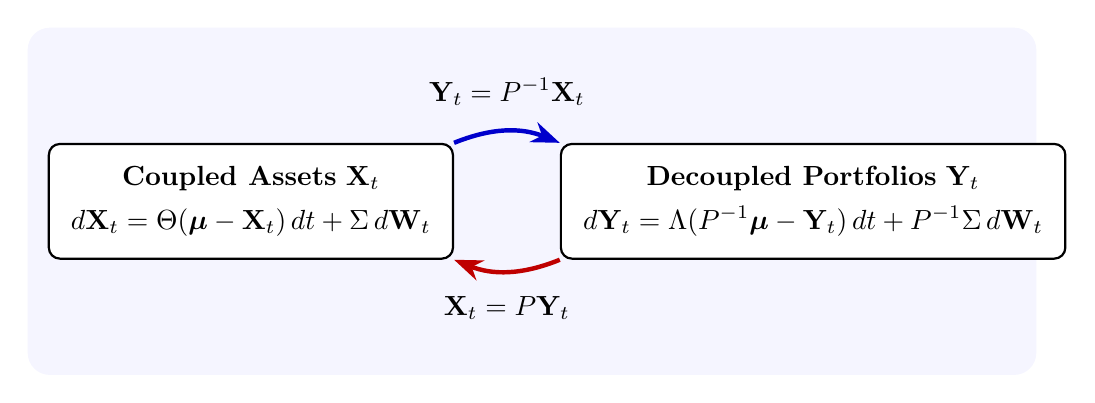
\begin{tikzpicture}[scale=1.05]
        % Layer 1: Background fill
        \fill[blue!4, rounded corners=8pt] (-6.1, -2.1) rectangle (6.1, 2.1);

        % Layer 2/3: System nodes and transformation arrows
        \node[draw=black, thick, fill=white, rounded corners=4pt, inner sep=8pt, text=black, align=center] (coupled) at (-3.4, 0)
            {\textbf{Coupled Assets} $\mathbf{X}_{t}$\\[4pt]
             $\displaystyle d\mathbf{X}_{t} = \Theta(\boldsymbol{\mu} - \mathbf{X}_{t})\,dt + \Sigma\,d\mathbf{W}_{t}$};

        \node[draw=black, thick, fill=white, rounded corners=4pt, inner sep=8pt, text=black, align=center] (decoupled) at (3.4, 0)
            {\textbf{Decoupled Portfolios} $\mathbf{Y}_{t}$\\[4pt]
             $\displaystyle d\mathbf{Y}_{t} = \Lambda(P^{-1}\boldsymbol{\mu} - \mathbf{Y}_{t})\,dt + P^{-1}\Sigma\,d\mathbf{W}_{t}$};

        \draw[->, >=Stealth, ultra thick, blue!80!black] (coupled.north east) to[bend left=22] node[midway, above=5pt, text=black] {$\displaystyle \mathbf{Y}_{t} = P^{-1}\mathbf{X}_{t}$} (decoupled.north west);

        \draw[->, >=Stealth, ultra thick, red!75!black] (decoupled.south west) to[bend left=22] node[midway, below=5pt, text=black] {$\displaystyle \mathbf{X}_{t} = P\mathbf{Y}_{t}$} (coupled.south east);
    \end{tikzpicture}
    \end{center}

    \item The second synthetic portfolio $Y_{t}^{(2)}$ mean-reverts $6$ times faster since $\lambda_{2} = 6 > \lambda_{1} = 1$. Its half-life of mean reversion is
    \[
    \tau_{1/2} = \frac{\ln 2}{6}.
    \]
\end{enumerate}

\vspace{0.8em}
\textbf{Problem 25 (Original Statement):}
Consider a two-asset Ornstein-Uhlenbeck model $d\mathbf{X}_{t} = \Theta(\boldsymbol{\mu} - \mathbf{X}_{t})\,dt + \Sigma\,d\mathbf{W}_{t}$ with non-symmetric drift matrix and correlated volatility:
\[
\Theta = \begin{bmatrix} 4 & -1 \\ 2 & 1 \end{bmatrix}, \qquad \boldsymbol{\mu} = \begin{bmatrix} 3 \\ 4 \end{bmatrix}, \qquad \Sigma = \begin{bmatrix} 2 & 1 \\ 1 & 2 \end{bmatrix}.
\]
\begin{enumerate}[label=(\alph*)]
    \item Diagonalize $\Theta = P\Lambda P^{-1}$ and explain why the eigenvalues confirm that the system is mean-reverting (stable).
    \item Transform the SDE to the eigenbasis $\mathbf{Y}_{t} = P^{-1}\mathbf{X}_{t}$ and compute the decoupled drift term $\Lambda(P^{-1}\boldsymbol{\mu} - \mathbf{Y}_{t})$ and transformed diffusion matrix $P^{-1}\Sigma$.
\end{enumerate}

\textbf{Solution:}
\begin{enumerate}[label=(\alph*)]
    \item Compute the characteristic polynomial of $\Theta$:
    \[
    \det(\Theta - \lambda I) = (4 - \lambda)(1 - \lambda) - (-1)(2) = \lambda^{2} - 5\lambda + 6 = (\lambda - 2)(\lambda - 3) = 0.
    \]
    The eigenvalues are $\lambda_{1} = 2$ and $\lambda_{2} = 3$.
    \begin{itemize}
        \item For $\lambda_{1} = 2$: $\Theta - 2I = \begin{bmatrix} 2 & -1 \\ 2 & -1 \end{bmatrix} \implies \mathbf{v}_{1} = \begin{bmatrix} 1 \\ 2 \end{bmatrix}$.
        \item For $\lambda_{2} = 3$: $\Theta - 3I = \begin{bmatrix} 1 & -1 \\ 2 & -2 \end{bmatrix} \implies \mathbf{v}_{2} = \begin{bmatrix} 1 \\ 1 \end{bmatrix}$.
    \end{itemize}
    Thus $P = \begin{bmatrix} 1 & 1 \\ 2 & 1 \end{bmatrix}$ ($\det(P) = -1$), $P^{-1} = \begin{bmatrix} -1 & 1 \\ 2 & -1 \end{bmatrix}$, and $\Lambda = \begin{bmatrix} 2 & 0 \\ 0 & 3 \end{bmatrix}$. Because both eigenvalues satisfy $\lambda_{i} > 0$, the negative-feedback drift $-\Lambda\mathbf{Y}_{t}$ decays deviations exponentially as $e^{-\lambda_{i} t}$, confirming stability and mean reversion.

    \item Compute the transformed equilibrium vector and diffusion matrix:
    \[
    P^{-1}\boldsymbol{\mu} = \begin{bmatrix} -1 & 1 \\ 2 & -1 \end{bmatrix}\begin{bmatrix} 3 \\ 4 \end{bmatrix} = \begin{bmatrix} 1 \\ 2 \end{bmatrix}, \qquad P^{-1}\Sigma = \begin{bmatrix} -1 & 1 \\ 2 & -1 \end{bmatrix}\begin{bmatrix} 2 & 1 \\ 1 & 2 \end{bmatrix} = \begin{bmatrix} -1 & 1 \\ 3 & 0 \end{bmatrix}.
    \]
    Thus the decoupled system is
    \[
    d\mathbf{Y}_{t} = \begin{bmatrix} 2 & 0 \\ 0 & 3 \end{bmatrix}\left(\begin{bmatrix} 1 \\ 2 \end{bmatrix} - \mathbf{Y}_{t}\right)dt + \begin{bmatrix} -1 & 1 \\ 3 & 0 \end{bmatrix}d\mathbf{W}_{t},
    \]
    whose drift terms $2(1 - Y_{t}^{(1)})$ and $3(2 - Y_{t}^{(2)})$ depend only on their respective synthetic components.
\end{enumerate}

\vspace{0.8em}
\textbf{Problem 26 (Original Statement):}
In Principal Component Analysis (PCA), a centered dataset in $\mathbb{R}^{2}$ has sample covariance matrix
\[
C = \begin{bmatrix} 5 & 2 \\ 2 & 2 \end{bmatrix}.
\]
\begin{enumerate}[label=(\alph*)]
    \item Diagonalize $C = PDP^{-1}$ such that the columns of $P$ are \emph{unit} eigenvectors $\{\mathbf{u}_{1}, \mathbf{u}_{2}\}$ ordered with $\lambda_{1} \ge \lambda_{2}$.
    \item What percentage of the total variance $\operatorname{tr}(C) = \lambda_{1} + \lambda_{2}$ is captured by the first principal component $\mathbf{u}_{1}$?
    \item Compute the principal component coordinates $[\mathbf{x}]_{\mathcal{B}} = P^{-1}\mathbf{x}$ of the observation $\mathbf{x} = \begin{bmatrix} 3 \\ 1 \end{bmatrix}$, and explain why $P^{-1} = P^{T}$ holds here.
\end{enumerate}

\textbf{Solution:}
\begin{enumerate}[label=(\alph*)]
    \item Find the eigenvalues of $C$:
    \[
    \det(C - \lambda I) = (5 - \lambda)(2 - \lambda) - 4 = \lambda^{2} - 7\lambda + 6 = (\lambda - 6)(\lambda - 1) = 0,
    \]
    so $\lambda_{1} = 6$ and $\lambda_{2} = 1$.
    \begin{itemize}
        \item For $\lambda_{1} = 6$: $C - 6I = \begin{bmatrix} -1 & 2 \\ 2 & -4 \end{bmatrix} \implies \mathbf{v}_{1} = \begin{bmatrix} 2 \\ 1 \end{bmatrix}$. Normalizing by $\|\mathbf{v}_{1}\| = \sqrt{2^{2}+1^{2}} = \sqrt{5}$ gives $\mathbf{u}_{1} = \frac{1}{\sqrt{5}}\begin{bmatrix} 2 \\ 1 \end{bmatrix}$.
        \item For $\lambda_{2} = 1$: $C - I = \begin{bmatrix} 4 & 2 \\ 2 & 1 \end{bmatrix} \implies \mathbf{v}_{2} = \begin{bmatrix} 1 \\ -2 \end{bmatrix}$. Normalizing by $\|\mathbf{v}_{2}\| = \sqrt{5}$ gives $\mathbf{u}_{2} = \frac{1}{\sqrt{5}}\begin{bmatrix} 1 \\ -2 \end{bmatrix}$.
    \end{itemize}
    Therefore,
    \[
    P = \frac{1}{\sqrt{5}}\begin{bmatrix} 2 & 1 \\ 1 & -2 \end{bmatrix}, \qquad D = \begin{bmatrix} 6 & 0 \\ 0 & 1 \end{bmatrix}.
    \]

    \item The total variance is $\operatorname{tr}(C) = \lambda_{1} + \lambda_{2} = 6 + 1 = 7$. The proportion of variance explained by the first principal component $\mathbf{u}_{1}$ is
    \[
    \frac{\lambda_{1}}{\lambda_{1} + \lambda_{2}} = \frac{6}{7} \approx 85.71\%.
    \]

    \item Because $C$ is a real symmetric matrix, eigenvectors corresponding to distinct eigenvalues are automatically orthogonal ($\mathbf{u}_{1} \cdot \mathbf{u}_{2} = 0$). Since both columns are also unit vectors, $P$ is an \emph{orthogonal matrix} ($P^{T}P = I$), which guarantees $P^{-1} = P^{T}$. Computing the eigenbasis coordinates of $\mathbf{x} = \begin{bmatrix} 3 \\ 1 \end{bmatrix}$:
    \[
    [\mathbf{x}]_{\mathcal{B}} = P^{T}\mathbf{x} = \frac{1}{\sqrt{5}}\begin{bmatrix} 2 & 1 \\ 1 & -2 \end{bmatrix}\begin{bmatrix} 3 \\ 1 \end{bmatrix} = \frac{1}{\sqrt{5}}\begin{bmatrix} 7 \\ 1 \end{bmatrix}.
    \]
    Geometrically, the orthogonal projection of $\mathbf{x}$ onto the first principal axis is $\left(\mathbf{u}_{1}^{T}\mathbf{x}\right)\mathbf{u}_{1} = \frac{7}{5}\begin{bmatrix} 2 \\ 1 \end{bmatrix} = \begin{bmatrix} 2.8 \\ 1.4 \end{bmatrix}$.

    \begin{center}
    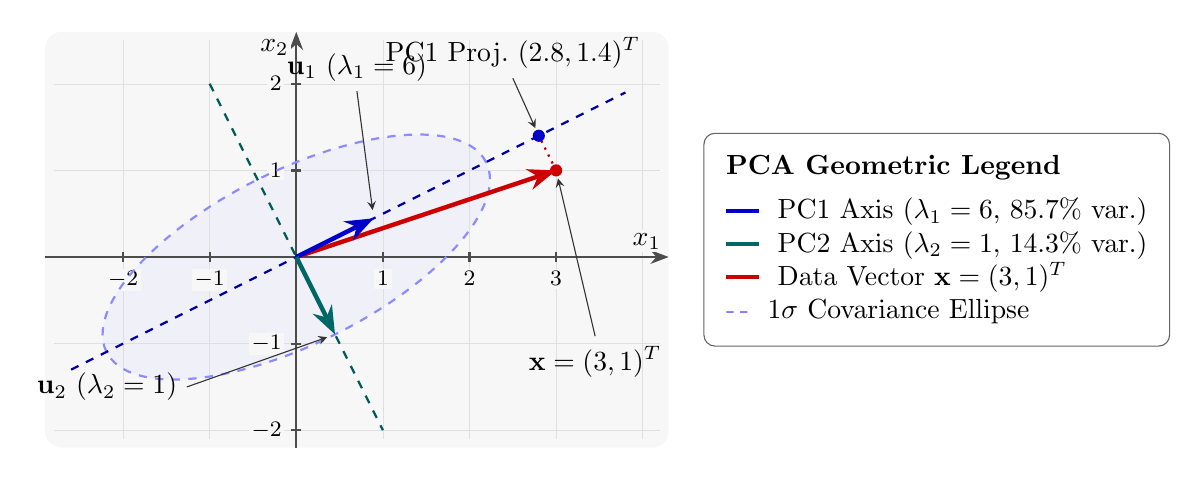
\begin{tikzpicture}[scale=1.1]
        % Layer 1: Background and shaded 1-sigma covariance ellipse
        \fill[gray!6, rounded corners=6pt] (-2.9, -2.2) rectangle (4.3, 2.6);
        \fill[blue!10, fill opacity=0.35, rotate around={26.565:(0,0)}] (0,0) ellipse (2.4495 and 1.0);

        % Layer 2: Grid and coordinate axes
        \draw[step=1, gray!25, very thin] (-2.8, -2.1) grid (4.2, 2.5);
        \draw[->, >=Stealth, thick, black!70] (-2.9, 0) -- (4.3, 0) node[above left=2pt, fill=gray!6, inner sep=1pt, text=black] {$x_{1}$};
        \draw[->, >=Stealth, thick, black!70] (0, -2.2) -- (0, 2.6) node[below left=2pt, fill=gray!6, inner sep=1pt, text=black] {$x_{2}$};
        \foreach \x in {-2,-1,1,2,3} {
            \draw[thick, black!70] (\x, 0.06) -- (\x, -0.06) node[below=2pt, fill=gray!6, inner sep=1pt, text=black] {\footnotesize $\x$};
        }
        \foreach \y in {-2,-1,1,2} {
            \draw[thick, black!70] (0.06, \y) -- (-0.06, \y) node[left=2pt, fill=gray!6, inner sep=1pt, text=black] {\footnotesize $\y$};
        }

        % Layer 3: Ellipse boundary, principal axes, vectors, and projection
        \draw[blue!45, thick, dashed, rotate around={26.565:(0,0)}] (0,0) ellipse (2.4495 and 1.0);
        \draw[blue!60!black, dashed, thick] (-2.6, -1.3) -- (3.8, 1.9);
        \draw[teal!70!black, dashed, thick] (-1.0, 2.0) -- (1.0, -2.0);
        \draw[red!70!black, dotted, thick] (3.0, 1.0) -- (2.8, 1.4);

        \draw[->, >=Stealth, ultra thick, red!80!black] (0, 0) -- (3.0, 1.0);
        \draw[->, >=Stealth, ultra thick, blue!80!black] (0, 0) -- (0.894, 0.447);
        \draw[->, >=Stealth, ultra thick, teal!80!black] (0, 0) -- (0.447, -0.894);

        \fill[red!80!black] (3.0, 1.0) circle (2pt);
        \fill[blue!80!black] (2.8, 1.4) circle (2pt);

        % Layer 4: Off-axis callouts and single-node multiline legend
        \node[text=black, above=2pt] (u1lbl) at (0.7, 1.85) {$\displaystyle \mathbf{u}_{1}\ (\lambda_{1} = 6)$};
        \draw[->, >=stealth, shorten >=3pt, black!80] (u1lbl.south) -- (0.894, 0.447);

        \node[text=black, left=2pt] (u2lbl) at (-1.2, -1.5) {$\displaystyle \mathbf{u}_{2}\ (\lambda_{2} = 1)$};
        \draw[->, >=stealth, shorten >=3pt, black!80] (u2lbl.east) -- (0.447, -0.894);

        \node[text=black, below=2pt] (xlbl) at (3.45, -0.85) {$\displaystyle \mathbf{x} = (3,1)^{T}$};
        \draw[->, >=stealth, shorten >=3pt, black!80] (xlbl.north) -- (3.0, 1.0);

        \node[text=black, above=2pt] (plbl) at (2.5, 2.0) {$\displaystyle \text{PC1 Proj.\ } (2.8, 1.4)^{T}$};
        \draw[->, >=stealth, shorten >=3pt, black!80] (plbl.south) -- (2.8, 1.4);

        \node[draw=black!60, fill=white, rounded corners=4pt, align=left, inner sep=8pt, anchor=west, text=black] at (4.7, 0.2) {%
            \textbf{PCA Geometric Legend}\\[4pt]
            \textcolor{blue!80!black}{\rule[0.5ex]{1.2em}{1.5pt}}\ \ PC1 Axis ($\lambda_{1} = 6$, $85.7\%$ var.)\\
            \textcolor{teal!80!black}{\rule[0.5ex]{1.2em}{1.5pt}}\ \ PC2 Axis ($\lambda_{2} = 1$, $14.3\%$ var.)\\
            \textcolor{red!80!black}{\rule[0.5ex]{1.2em}{1.5pt}}\ \ Data Vector $\mathbf{x} = (3,1)^{T}$\\
            \textcolor{blue!60}{-\,-}\ \ $1\sigma$ Covariance Ellipse
        };
    \end{tikzpicture}
    \end{center}
\end{enumerate}

\subsection{Solutions to Part G: Diagnostic Error Analysis (``Find the Flaw'')}

\textbf{Problem 27 (Original Statement):}
Act as the grader for the following attempt to compute $A^{2}$ for $A = \begin{bmatrix} 1 & 2 \\ 4 & 3 \end{bmatrix}$ via diagonalization:
\begin{quote}
\emph{Student's Solution:} Solving $\det(A - \lambda I) = 0$ gives $\lambda_{1} = 5$ with eigenvector $\mathbf{v}_{1} = \begin{bmatrix} 1 \\ 2 \end{bmatrix}$ and $\lambda_{2} = -1$ with eigenvector $\mathbf{v}_{2} = \begin{bmatrix} 1 \\ -1 \end{bmatrix}$. Forming
\[
P = \begin{bmatrix} 1 & 1 \\ -1 & 2 \end{bmatrix}, \qquad D = \begin{bmatrix} 5 & 0 \\ 0 & -1 \end{bmatrix},
\]
and inverting $P$ gives $P^{-1} = \begin{bmatrix} 2 & -1 \\ 1 & 1 \end{bmatrix}$. Hence
\[
A^{2} = PD^{2}P^{-1} = \begin{bmatrix} 1 & 1 \\ -1 & 2 \end{bmatrix} \begin{bmatrix} 25 & 0 \\ 0 & 1 \end{bmatrix} \begin{bmatrix} 2 & -1 \\ 1 & 1 \end{bmatrix} = \begin{bmatrix} 51 & -24 \\ -48 & 27 \end{bmatrix}.
\]
\end{quote}
Identify \textbf{two} distinct flaws in the student's work, explain why each is incorrect, and compute the correct diagonalization and value of $A^{2}$.

\textbf{Solution:}
\textbf{Flaw 1 (Mismatched Order):} The student placed $\mathbf{v}_{2}$ in column $1$ of $P$ and $\mathbf{v}_{1}$ in column $2$ of $P$, while placing $\lambda_{1} = 5$ in column $1$ of $D$ and $\lambda_{2} = -1$ in column $2$ of $D$; the order of eigenvectors in $P$ must match the order of eigenvalues in $D$.

\textbf{Flaw 2 (Missing $1/\det(P)$ Factor):} When inverting $P$, the student swapped the diagonal entries and negated the off-diagonal entries but forgot to divide by $\det(P)$.

\textbf{Correct Computation:} Aligning the columns of $P$ with $D$:
\[
P = \begin{bmatrix} 1 & 1 \\ 2 & -1 \end{bmatrix}, \qquad D = \begin{bmatrix} 5 & 0 \\ 0 & -1 \end{bmatrix}.
\]
Since $\det(P) = (1)(-1) - (1)(2) = -3$, the true inverse is
\[
P^{-1} = \frac{1}{-3}\begin{bmatrix} -1 & -1 \\ -2 & 1 \end{bmatrix} = \frac{1}{3}\begin{bmatrix} 1 & 1 \\ 2 & -1 \end{bmatrix}.
\]
Then $D^{2} = \begin{bmatrix} 25 & 0 \\ 0 & 1 \end{bmatrix}$, and
\[
A^{2} = PD^{2}P^{-1} = \frac{1}{3}\begin{bmatrix} 25 & 1 \\ 50 & -1 \end{bmatrix}\begin{bmatrix} 1 & 1 \\ 2 & -1 \end{bmatrix} = \frac{1}{3}\begin{bmatrix} 27 & 24 \\ 48 & 51 \end{bmatrix} = \begin{bmatrix} 9 & 8 \\ 16 & 17 \end{bmatrix}.
\]

\vspace{0.8em}
\textbf{Problem 28 (Original Statement):}
Act as the grader for the following attempt to diagonalize $A = \begin{bmatrix} 3 & 2 \\ 5 & 0 \end{bmatrix}$ over $\mathbb{R}$:
\begin{quote}
\emph{Student's Solution:} The characteristic equation is $\det(A - \lambda I) = (3 - \lambda)(-\lambda) + (2)(5) = \lambda^{2} - 3\lambda + 10 = 0$. Since the discriminant is $(-3)^{2} - 4(1)(10) = -31 < 0$, $A$ has no real eigenvalues and therefore cannot be diagonalized over $\mathbb{R}$.
\end{quote}
Identify the flaw, explain why it is incorrect in one sentence, and find the correct eigenvalues and diagonalization $P, D$.

\textbf{Solution:}
\textbf{Flaw \& Correction:} Because the determinant of a $2 \times 2$ matrix $\begin{bmatrix} a & b \\ c & d \end{bmatrix}$ is $ad - bc$, the student erroneously added the off-diagonal product $(2)(5)$ instead of subtracting it.

\textbf{Correct Computation:}
\[
\det(A - \lambda I) = (3 - \lambda)(-\lambda) - (2)(5) = \lambda^{2} - 3\lambda - 10 = (\lambda - 5)(\lambda + 2) = 0,
\]
giving distinct real eigenvalues $\lambda_{1} = 5$ and $\lambda_{2} = -2$.
\begin{itemize}
    \item For $\lambda_{1} = 5$: $A - 5I = \begin{bmatrix} -2 & 2 \\ 5 & -5 \end{bmatrix} \implies \mathbf{v}_{1} = \begin{bmatrix} 1 \\ 1 \end{bmatrix}$.
    \item For $\lambda_{2} = -2$: $A + 2I = \begin{bmatrix} 5 & 2 \\ 5 & 2 \end{bmatrix} \implies \mathbf{v}_{2} = \begin{bmatrix} 2 \\ -5 \end{bmatrix}$.
\end{itemize}
\textbf{Correct Answer:} $P = \begin{bmatrix} 1 & 2 \\ 1 & -5 \end{bmatrix}$ and $D = \begin{bmatrix} 5 & 0 \\ 0 & -2 \end{bmatrix}$.

\vspace{0.8em}
\textbf{Problem 29 (Original Statement):}
Act as the grader for the following computation of $A^{3}$ given $A = PDP^{-1}$ with $P = \begin{bmatrix} 1 & 1 \\ 0 & 1 \end{bmatrix}$ and $D = \begin{bmatrix} 2 & 0 \\ 0 & 3 \end{bmatrix}$:
\begin{quote}
\emph{Student's Solution:} Raising the factorization to the third power gives
\[
A^{3} = P^{-1}D^{3}P = \begin{bmatrix} 1 & -1 \\ 0 & 1 \end{bmatrix} \begin{bmatrix} 8 & 0 \\ 0 & 27 \end{bmatrix} \begin{bmatrix} 1 & 1 \\ 0 & 1 \end{bmatrix} = \begin{bmatrix} 8 & -19 \\ 0 & 27 \end{bmatrix}.
\]
\end{quote}
Identify the flaw, explain why it is incorrect in one sentence, and compute the correct matrix $A^{3}$.

\textbf{Solution:}
\textbf{Flaw \& Correction:} Matrix multiplication is non-commutative, and telescoping cancellation yields $A^{3} = (PDP^{-1})(PDP^{-1})(PDP^{-1}) = PD^{3}P^{-1}$ with $P$ on the left and $P^{-1}$ on the right, not the reverse.

\textbf{Correct Computation:}
\[
A^{3} = PD^{3}P^{-1} = \begin{bmatrix} 1 & 1 \\ 0 & 1 \end{bmatrix}\begin{bmatrix} 8 & 0 \\ 0 & 27 \end{bmatrix}\begin{bmatrix} 1 & -1 \\ 0 & 1 \end{bmatrix} = \begin{bmatrix} 8 & 27 \\ 0 & 27 \end{bmatrix}\begin{bmatrix} 1 & -1 \\ 0 & 1 \end{bmatrix} = \begin{bmatrix} 8 & 19 \\ 0 & 27 \end{bmatrix}.
\]

\vspace{0.8em}
\textbf{Problem 30 (Original Statement):}
Act as the grader for the following attempt to determine whether $A = \begin{bmatrix} 4 & 1 \\ -1 & 2 \end{bmatrix}$ is diagonalizable:
\begin{quote}
\emph{Student's Solution:} We find $\det(A - \lambda I) = (4-\lambda)(2-\lambda) + 1 = (\lambda - 3)^{2} = 0$, so $\lambda = 3$ has algebraic multiplicity $2$. Solving $(A - 3I)\mathbf{x} = \mathbf{0}$ yields $\mathbf{v}_{1} = \begin{bmatrix} 1 \\ -1 \end{bmatrix}$. Choosing a second eigenvector $\mathbf{v}_{2} = \begin{bmatrix} -2 \\ 2 \end{bmatrix}$ gives
\[
P = \begin{bmatrix} 1 & -2 \\ -1 & 2 \end{bmatrix}, \qquad D = \begin{bmatrix} 3 & 0 \\ 0 & 3 \end{bmatrix},
\]
so $A$ is diagonalizable.
\end{quote}
Identify the flaw, explain why it is incorrect, and state the correct conclusion regarding the diagonalizability of $A$.

\textbf{Solution:}
\textbf{Flaw \& Correction:} Diagonalizability requires $P$ to be \emph{invertible}, which means its columns must be \emph{linearly independent} eigenvectors; because $\mathbf{v}_{2} = -2\mathbf{v}_{1}$ is a scalar multiple of $\mathbf{v}_{1}$, the columns of $P$ are linearly dependent and $\det(P) = (1)(2) - (-2)(-1) = 0$, so $P^{-1}$ does not exist.

\textbf{Correct Conclusion:} Since $A - 3I = \begin{bmatrix} 1 & 1 \\ -1 & -1 \end{bmatrix}$ has rank $1$, the eigenspace $\operatorname{Nul}(A - 3I)$ has geometric multiplicity $2 - 1 = 1 < 2$. Therefore, $A$ is \textbf{defective and not diagonalizable}.

\newpage
\section{Concept Checklist and Question Reference}

For rapid review after practice, the table below repeats the complete concept checklist and maps each problem type, shortcut, pitfall, and application back to its exact question numbers in this packet.

\renewcommand{\arraystretch}{1.5}
\begin{tabularx}{\textwidth}{l X X c p{3.1cm}}
\toprule
\textbf{ID} & \textbf{Concept / Problem Type} & \textbf{Key Techniques, Theorems, and Pitfalls} & \textbf{Weight} & \textbf{Relevant Questions} \\
\midrule
C1 & Matrix Powers via Factorization ($A^{k} = PD^{k}P^{-1}$) & $2 \times 2$ inverse with $1/\det(P)$, telescoping cancellation, symbolic powers, asymptotic limits. & 4 (13.3\%) & \textbf{Primary:} \hyperref[prob:1]{1}, \hyperref[prob:2]{2}, \hyperref[prob:3]{3}, \hyperref[prob:4]{4}\newline \textbf{Related:} \hyperref[prob:20]{20}, \hyperref[prob:23]{23}, \hyperref[prob:29]{29} \\
\addlinespace[3pt]
C2 & Triangular Shortcuts and Fraction Avoidance & Reading $\lambda$ directly off triangular diagonals; scaling free variables to avoid fractions in RREF. & 2 (6.7\%) & \textbf{Primary:} \hyperref[prob:5]{5}, \hyperref[prob:6]{6}\newline \textbf{Related:} \hyperref[prob:8]{8}, \hyperref[prob:11]{11}, \hyperref[prob:14]{14}, \hyperref[prob:15]{15} \\
\addlinespace[3pt]
C3 & Full Diagonalization ($2 \times 2$ and $3 \times 3$) & Solving $\det(A-\lambda I)=0$, computing bases for $\operatorname{Nul}(A-\lambda I)$, handling $\lambda = 0$ and repeated $\lambda$. & 5 (16.7\%) & \textbf{Primary:} \hyperref[prob:7]{7}, \hyperref[prob:8]{8}, \hyperref[prob:9]{9}, \hyperref[prob:10]{10}, \hyperref[prob:11]{11}\newline \textbf{Related:} \hyperref[prob:4]{4}, \hyperref[prob:22]{22}--\hyperref[prob:26]{26} \\
\addlinespace[3pt]
C4 & Conceptual Theorems and Parametric Analysis & Theorems 5, 6, 7; similarity vs.\ diagonalizability; rank-nullity; parameter conditions for diagonalizability. & 4 (13.3\%) & \textbf{Primary:} \hyperref[prob:12]{12}, \hyperref[prob:13]{13}, \hyperref[prob:14]{14}, \hyperref[prob:15]{15}\newline \textbf{Related:} \hyperref[prob:21]{21}, \hyperref[prob:30]{30} \\
\addlinespace[3pt]
C5 & Defective Matrices and Jordan Canonical Form & Algebraic vs.\ geometric multiplicity gap, $\det(P)=0$ failure, nilpotent blocks $A = \lambda I + N$ and $J$. & 3 (10.0\%) & \textbf{Primary:} \hyperref[prob:16]{16}, \hyperref[prob:17]{17}, \hyperref[prob:18]{18}\newline \textbf{Related:} \hyperref[prob:14]{14}, \hyperref[prob:15]{15}, \hyperref[prob:30]{30} \\
\addlinespace[3pt]
C6 & Change of Basis, Matrix Roots, and Structural Identities & Computing $A^{k}\mathbf{x}$ via $[\mathbf{x}]_{\mathcal{B}}$, reconstructing $A$, $A^{-1}$, $\sqrt{A}$, $A^{T}$, and $A+cI$. & 3 (10.0\%) & \textbf{Primary:} \hyperref[prob:19]{19}, \hyperref[prob:20]{20}, \hyperref[prob:21]{21}\newline \textbf{Related:} \hyperref[prob:24]{24}, \hyperref[prob:26]{26} \\
\addlinespace[3pt]
C7 & Applied Decoupling (ODEs, Recurrences, OU, PCA) & Coupled $\mathbf{x}' = A\mathbf{x}$, discrete $\mathbf{x}_{k+1}=A\mathbf{x}_k$, Ornstein-Uhlenbeck SDEs ($\mathbf{Y}_t = P^{-1}\mathbf{X}_t$), PCA variance. & 5 (16.7\%) & \textbf{Primary:} \hyperref[prob:22]{22}, \hyperref[prob:23]{23}, \hyperref[prob:24]{24}, \hyperref[prob:25]{25}, \hyperref[prob:26]{26}\newline \textbf{Related:} \hyperref[prob:4]{4} \\
\addlinespace[3pt]
C8 & Diagnostic Error Analysis (``Find the Flaw'') & Detecting swapped columns in $P$/$D$, $ad+bc$ sign errors, $P^{-1}D^{k}P$ order errors, missing $1/\det(P)$, repeated vectors. & 4 (13.3\%) & \textbf{Primary:} \hyperref[prob:27]{27}, \hyperref[prob:28]{28}, \hyperref[prob:29]{29}, \hyperref[prob:30]{30}\newline \textbf{Related:} \hyperref[prob:12]{12} \\
\bottomrule
\end{tabularx}

\end{document}